\documentclass[aspectratio=169]{beamer}

\usepackage[english]{babel}
\usepackage[T1]{fontenc}
\usepackage{amsmath, amssymb, amsthm}
\usepackage{graphicx}
\usepackage{booktabs}
\usepackage{xcolor}
\usepackage{bm}
\usepackage{tikz}
\usetikzlibrary{arrows.meta,positioning,fit}
\usepackage{animate}

\graphicspath{{../../plots/}{../text/}}

\definecolor{polybleu}{RGB}{0,62,92}
\definecolor{polyrouge}{RGB}{213,43,30}
\definecolor{polybleuclair}{RGB}{0,104,128}

\mode<presentation>
{
  \usetheme{Madrid}
  \usecolortheme[named=polybleu]{structure}
  \setbeamercolor{palette primary}{bg=polybleu,fg=white}
  \setbeamercolor{palette secondary}{bg=polybleuclair,fg=white}
  \setbeamercolor{palette tertiary}{bg=polybleu,fg=white}
  \setbeamercolor{palette quaternary}{bg=polybleu,fg=white}
  \setbeamercolor{titlelike}{parent=palette primary,bg=white,fg=polybleu}
  \setbeamercolor{item}{fg=polyrouge}
  \setbeamertemplate{navigation symbols}{}
  \setbeamertemplate{caption}[numbered]
  
  \useinnertheme{rectangles}
}

\title[Offline Laplace Order Reduction]{Offline Laplace-Domain Order Reduction for Complex Convection-Diffusion-Reaction Dynamics}
\subtitle{From Proper Orthogonal Decomposition to Frequency-Conditioned Autoencoders}
\author[Keyvan Attarian]{Keyvan Attarian}
\institute[Ecole polytechnique]{Ecole polytechnique \\ CNRS@CREATE - DesCartes Program}
\date{\today}

\titlegraphic{%
  
\includegraphics[height=1.2cm]{polytechnique-logohori.pdf}\hfill
  
\includegraphics[height=1.2cm]{logodescartes.png}
}

\newcommand{\vtheta}{\bm{\theta}}
\newcommand{\R}{\mathbb{R}}
\newcommand{\C}{\mathbb{C}}
\newcommand{\E}{\mathbb{E}}

\begin{document}

{
\usebackgroundtemplate{%
  \tikz[overlay,remember picture] \node[opacity=0.15, at=(current page.center)] {
\includegraphics[height=0.8\paperheight]{polytechnique-armes.pdf}};%
}
\begin{frame}
  \titlepage
\end{frame}
}

\begin{frame}{Outline}
  \tableofcontents
\end{frame}

\section{Introduction}

\begin{frame}{Preliminary Study: 2D Convection-Diffusion Dataset}
  \textbf{Physical Problem:} Stationary convection-diffusion on $\Omega = [0,1]^2$
  \begin{equation*}
      -D\,\Delta U + \bm{b} \cdot \nabla U = f \qquad \text{with } U=0 \text{ on } \partial\Omega
  \end{equation*}
  
  \begin{itemize}
      \item \textbf{Parameters:} $\vtheta = (D, b_x, b_y, f) \in \mathbb{R}^4$ (diffusivity, velocity, source).
      \item \textbf{Dataset Generation:} 10,000 simulations solved via P1 finite elements.
      \item \textbf{Format:} Solutions interpolated to a uniform $N \times N$ grid.
  \end{itemize}
  
  \begin{figure}
      \centering
      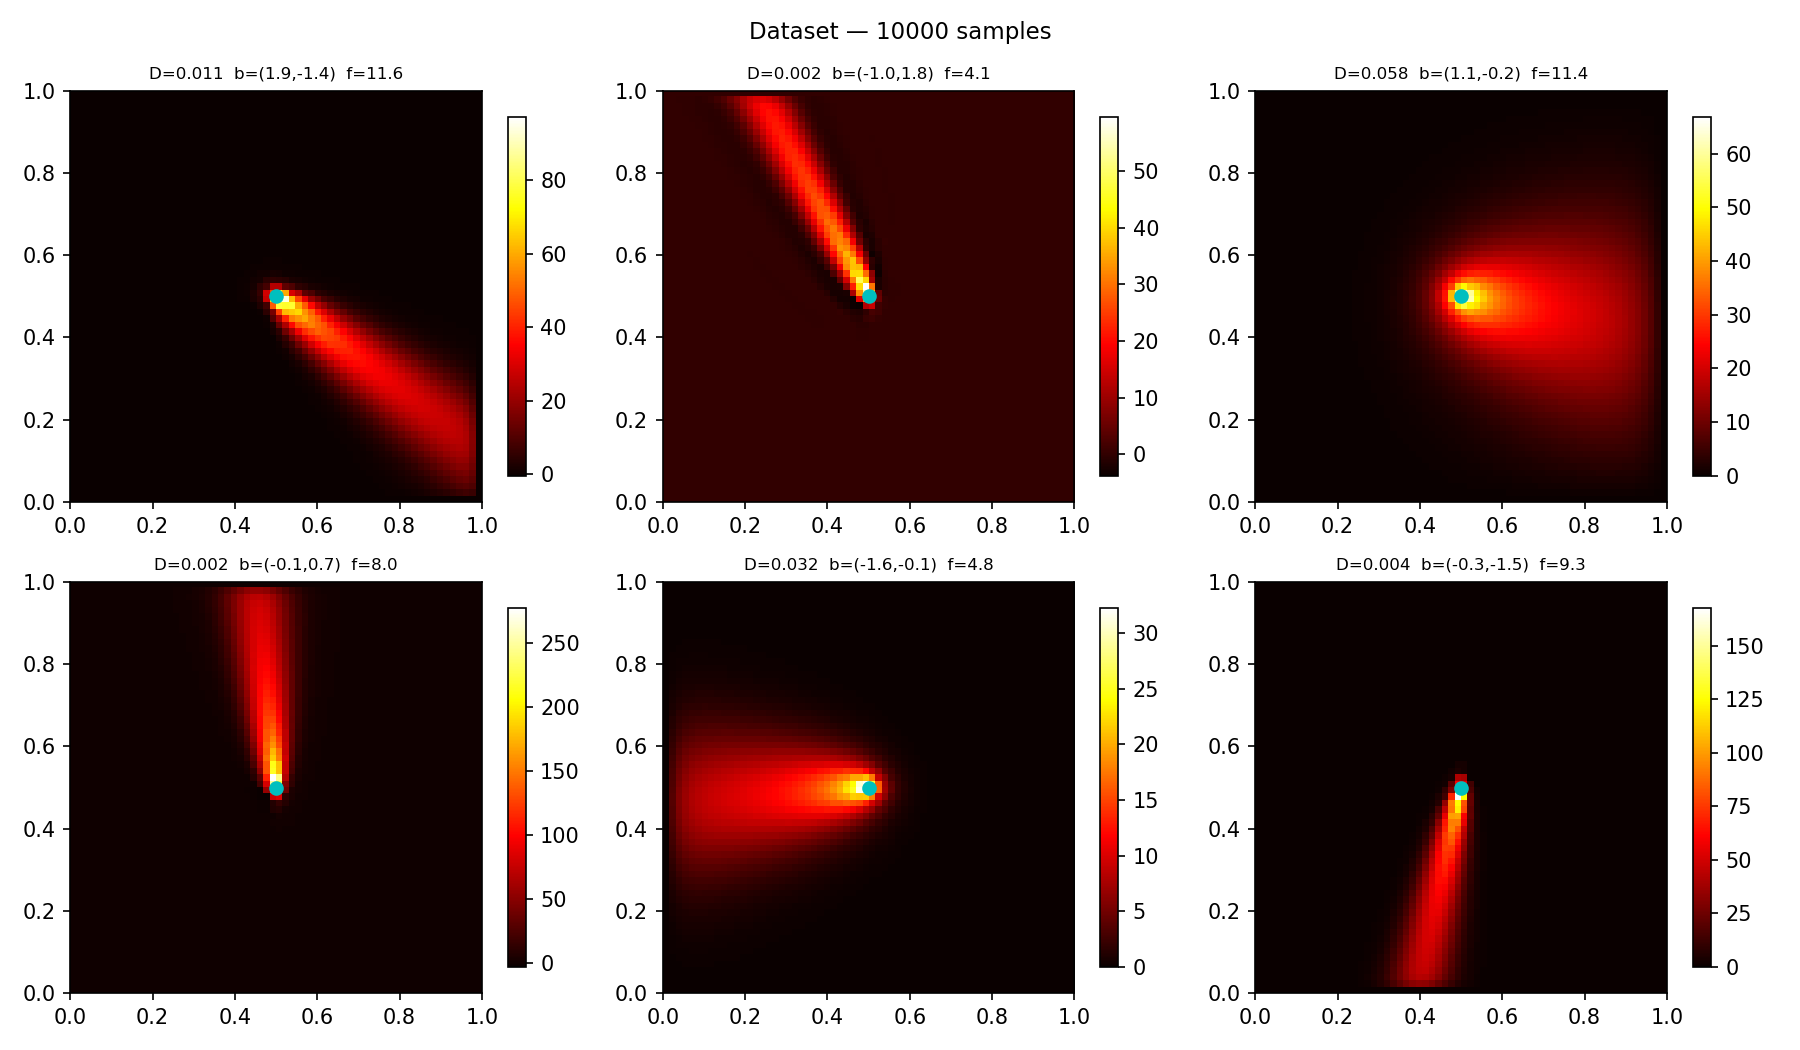
\includegraphics[width=0.95\textwidth, height=4.2cm, keepaspectratio]{dataset_preview.png}
      \caption{Stationary convection-diffusion dataset preview}
  \end{figure}
\end{frame}

\begin{frame}{Preliminary Study: Latent Surrogate Strategy}
  \textbf{Method:} Two-stage Variational Autoencoder (VAE) backbone.
  \begin{enumerate}
      \item \textbf{Representation:} VAE ($U \to z \to \hat{U}$)
      \item \textbf{Regression:} MLP surrogate ($\vtheta \to z$)
  \end{enumerate}
  
  \vspace{0.3em}
  \textbf{Bottleneck: The frozen spatial representation}
  \begin{columns}[T]
      \column{0.48\textwidth}
      \begin{itemize}
          \item \textbf{Frozen Decoder:} Rigid latent space yields poor accuracy (\textbf{27.7\%} error).
      \end{itemize}
      \column{0.48\textwidth}
      \begin{itemize}
          \item \textbf{End-to-End Fine-Tuning:} Unlocking decoder drops error to \textbf{9.9\%} (VAE floor: 8.1\%).
      \end{itemize}
  \end{columns}
  
  \begin{figure}
      \centering
      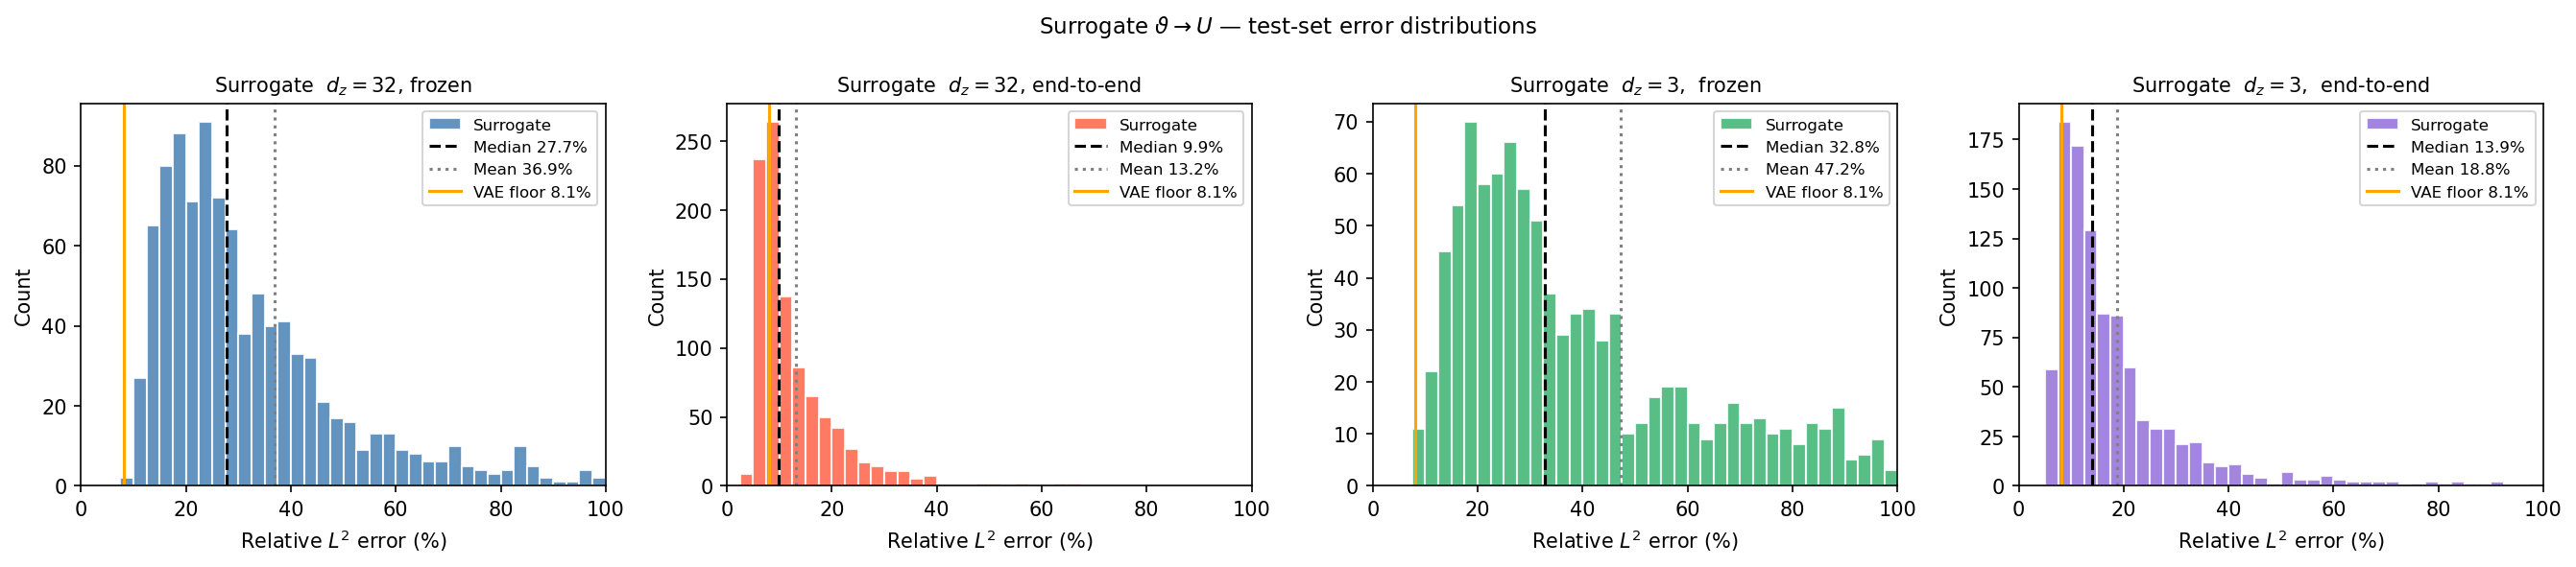
\includegraphics[width=0.8\textwidth]{surrogate_l2rel_hist.png}
      \caption{Surrogate L2 relative error}
  \end{figure}
\end{frame}

\section{The Transient Challenge}

\begin{frame}{The Transient Problem}
  \textbf{Dataset: Atmospheric Methane (CH$_4$) Dispersion}
  \begin{itemize}
      \item 8,100 simulations, 150 snapshots on $200 \times 200$ grid.
      \item Parameters: $\vtheta = (k, A, C)$ (reaction rate, angle, concentration).
  \end{itemize}
  \begin{figure}
      \centering
      \animategraphics[loop,autoplay,width=0.9\textwidth]{10}{frames_ch4_demo/frame_}{0}{74}
      \caption{Methane dispersion demonstration}
  \end{figure}
  \vspace{0.5em}
  \textbf{Challenge:} High dimensionality $(150 \times 200^2)$ makes direct regression intractable.
\end{frame}

\begin{frame}{Linear Baseline 1: Tucker POD}
  \begin{columns}
      \column{0.5\textwidth}
      \begin{itemize}
          \item \textbf{Method:} Tucker decomposition into separable $(F, P, G)$ modes:
          \[ H(x, t; \vtheta) \approx \sum_{j=1}^{n_f} \alpha_j\, F_j(x)\, P_j(t)\, G_j(\vtheta) \]
          \item \textbf{Memory Bottleneck:} Requires holding the full tensor in RAM. Forces severe spatial downsampling from $200 \times 200$ to $40 \times 40$.
          \item \textbf{Performance:} Reaches an irreducible $\sim$10\% reconstruction floor.
      \end{itemize}
      \column{0.5\textwidth}
      \begin{figure}
          \centering
          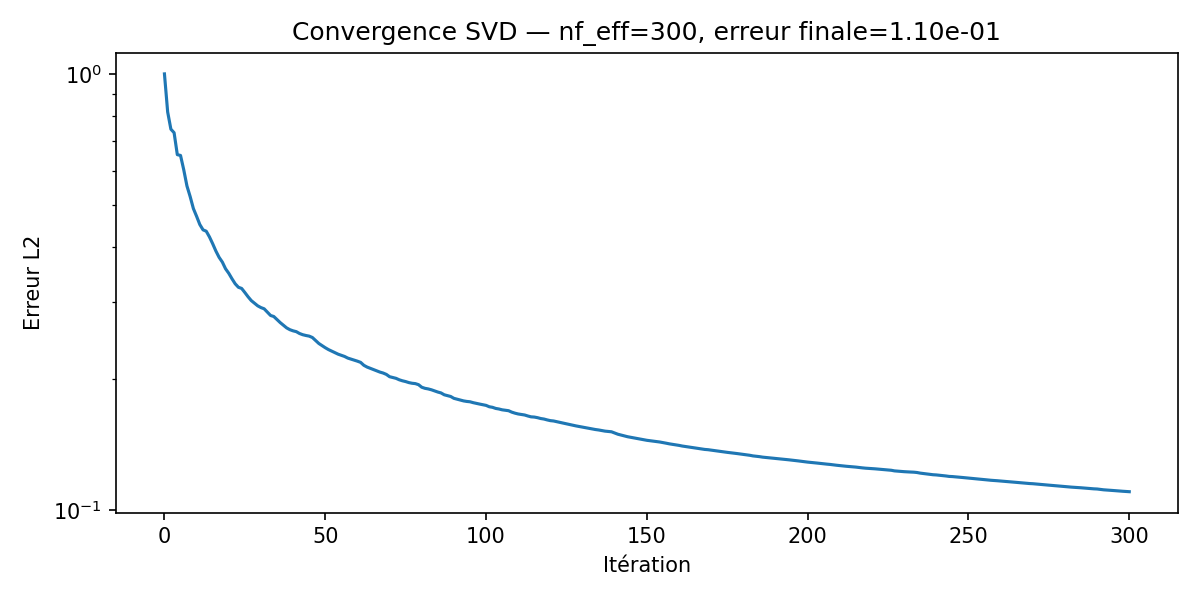
\includegraphics[height=2.5cm]{svd_convergence.png}
          \caption{SVD convergence}
      \end{figure}
      \vspace{-0.5em}
      \begin{figure}
          \centering
          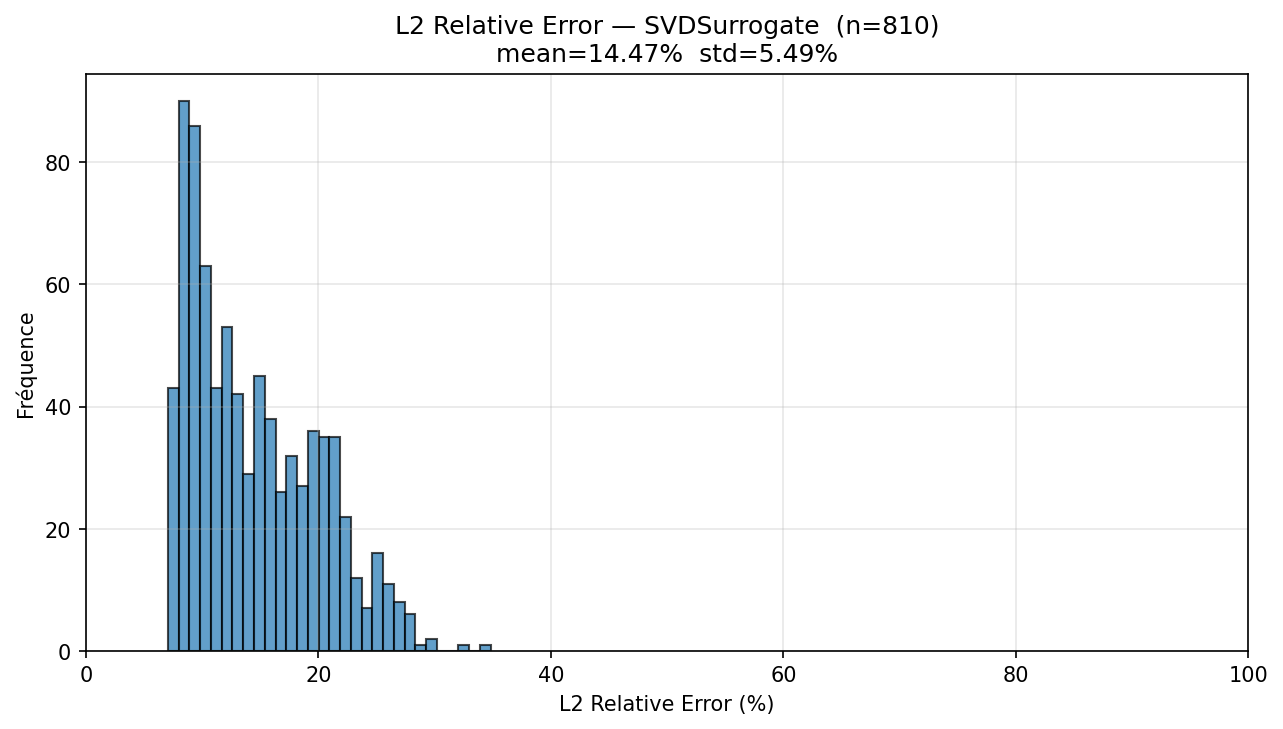
\includegraphics[height=2.5cm]{SVDSurrogate_l2rel_hist.png}
          \caption{SVD Surrogate Error}
      \end{figure}
  \end{columns}
\end{frame}

\section{The Laplace Transformation}

\begin{frame}{Temporal Decoupling: The Laplace Domain}
  Transform temporal fields via \textbf{discrete Bromwich integral}:
  \[
    \hat{U}(s_k) = \int_0^T U(t)\,e^{-s_k t}\,\mathrm{d}t \;\approx\; \Delta t \sum_{n=0}^{N_t-1} w_n\, U_n\, e^{-\gamma t_n} e^{-i\omega_k t_n}
  \]
  \begin{columns}
      \column{0.5\textwidth}
      \begin{itemize}
          \item Converts 3D transient fields into 2D independent stationary-like complex fields.
          \item Spectrum drops rapidly: truncated at $k_{\max} = 20$.
          \item Differentiable transform: allows processing at \textbf{full spatial resolution}.
      \end{itemize}
      \column{0.5\textwidth}
      \begin{figure}
          \centering
          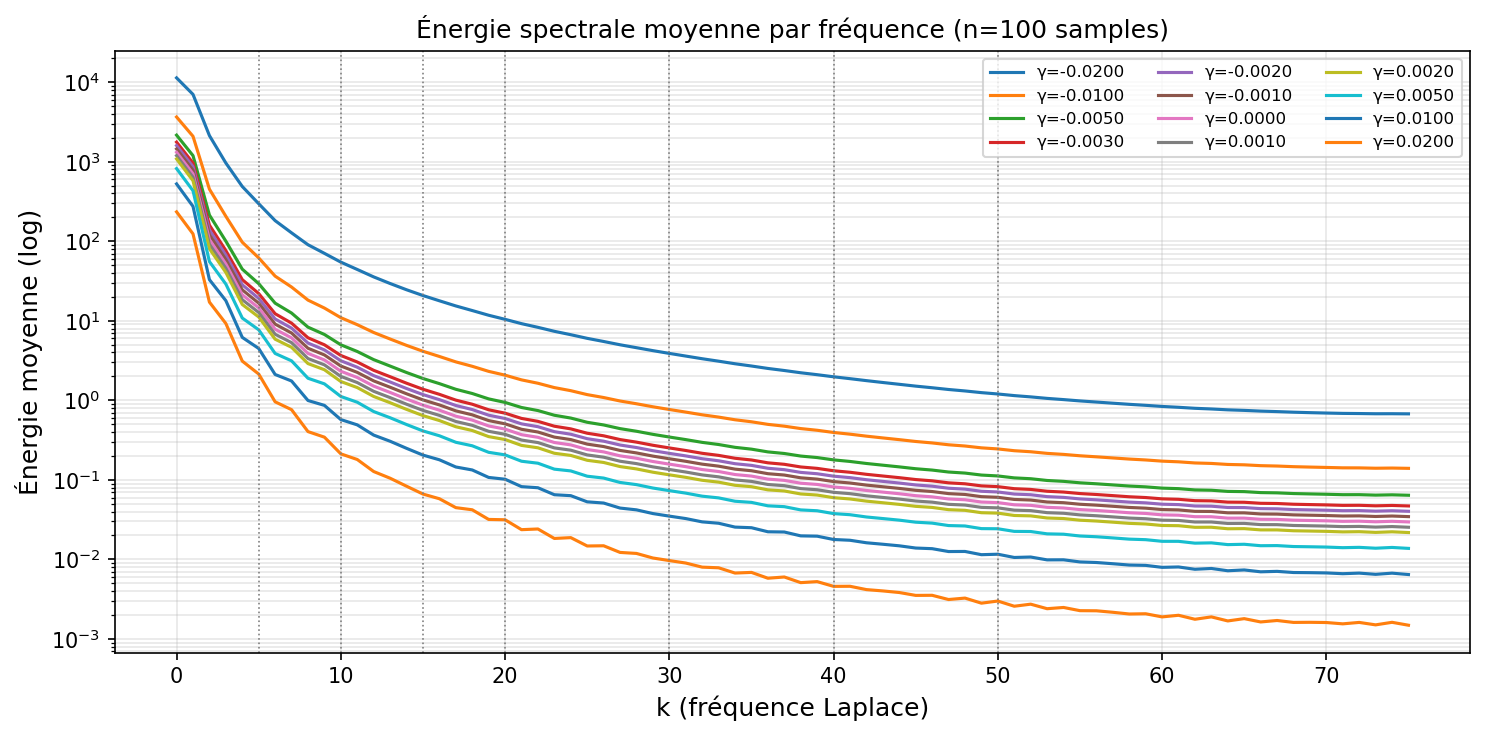
\includegraphics[width=0.85\linewidth]{gamma_opti_energy.png}
          \caption{Gamma optimization energy}
      \end{figure}
  \end{columns}
\end{frame}

\begin{frame}{Linear Baseline 2: SVD in Laplace Domain}
  What if we apply SVD on independent complex 2D frequency slices?
  \vspace{0.5em}
  \begin{columns}[T]
      \column{0.48\textwidth}
      \begin{itemize}
          \item \textbf{Method:} Truncated SVD per frequency. MLPs regress parameters into spatial bases:
          \[ \hat{U}_k(x; \vtheta) \approx \sum_{j=1}^{k_{\mathrm{svd}}} c_j^{(k)}(\vtheta)\, V_j^{(k)}(x) \]
      \end{itemize}
      
      \column{0.48\textwidth}
      \begin{itemize}
          \item \textbf{Limitation:} High truncation error growing monotonically.
          \item \textbf{Conclusion:} Fixed linear bases yield noisy targets, motivating non-linear autoencoders.
      \end{itemize}
  \end{columns}
  
  \begin{figure}
      \centering
      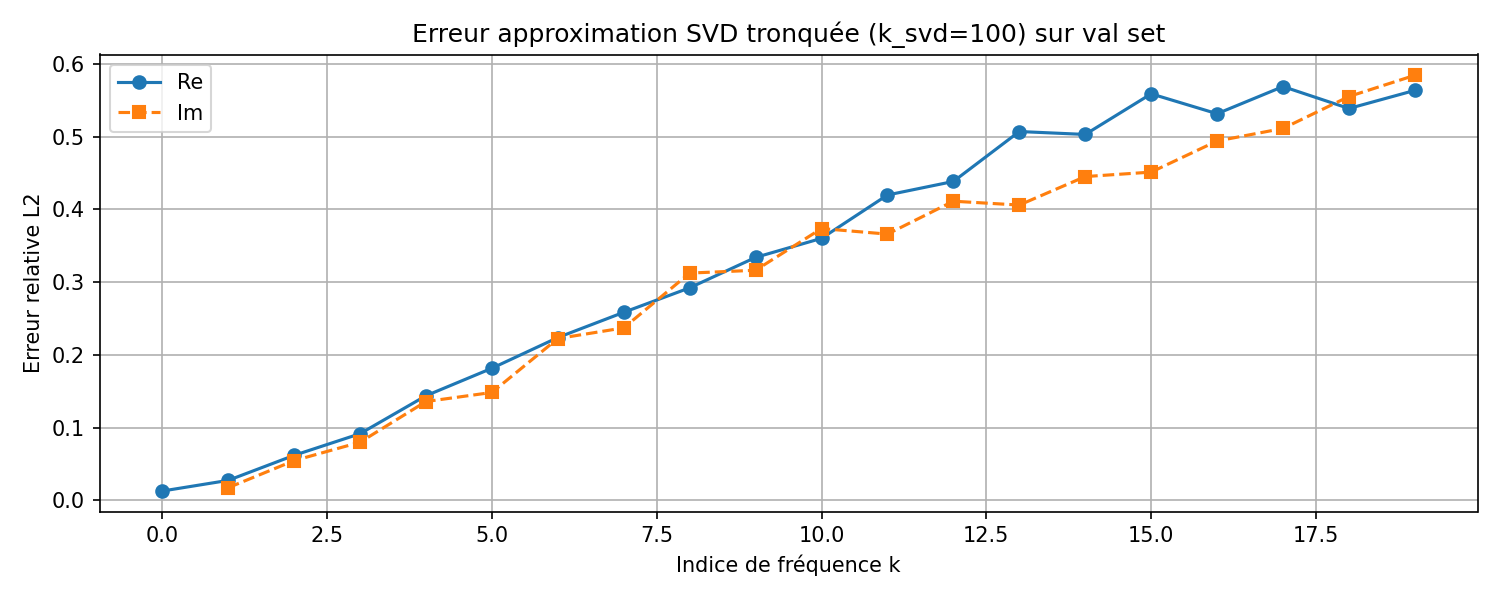
\includegraphics[height=3.0cm]{LaplaceSVDModel_svd_error_ksvd100.png}
      \caption{Laplace SVD Model error}
  \end{figure}
\end{frame}

\section{Latent Space Pipeline}

\begin{frame}{Latent Space Structure: Autoencoder Architecture}
  To handle multiple complex frequencies continuously, we employ a conditional convolutional architecture:
  \vspace{0.5em}
  \begin{itemize}
      \item \textbf{Frequency Conditioning:} The target frequency ratio $f_k = k/(N_{\mathrm{half}}-1) \in [0,1]$ is embedded via a multi-scale sinusoidal basis:
      \[ \bm{e}(f_k) = \mathrm{MLP}\Bigl(\bigl[\sin(2^i\pi f_k),\; \cos(2^i\pi f_k)\bigr]_{i=0}^{L-1}\Bigr) \]
      \item \textbf{FiLM Modulation:} The embedded feature $\bm{e}(f_k)$ is projected to channel-wise gains $\alpha_\ell$ and biases $\delta_\ell$, modulating the activation maps $\bm{x}_\ell$ at each layer $\ell$:
      \[ \bm{x}_\ell \;\leftarrow\; \bigl(\bm{x}_\ell \odot (1 + \alpha_\ell(\bm{e}(f_k)))\bigr) \;+\; \delta_\ell(\bm{e}(f_k)) \]
      The residual gain formulation $(1 + \alpha_\ell)$ stabilises early training.
      \item \textbf{Architecture:} A shared CNN processes all frequency slices, defining a mapped latent space:
      \[ z = \mathrm{Enc}_\phi(\hat{U}_k, f_k), \quad \tilde{U}_k = \mathrm{Dec}_\psi(z, f_k) \]
  \end{itemize}
\end{frame}

\begin{frame}{Latent Space: Shared Architecture and Temporal Error}
  We train a \textbf{single shared autoencoder} using \textbf{FiLM modulation} and \textbf{Sinusoidal Encodings}.
  \vspace{1em}
  
  Temporal inversion yields a \textbf{9.94\% mean error floor}.
  \vspace{0.5em}

  \begin{columns}
      \column{0.5\textwidth}
      \begin{figure}
          \centering
          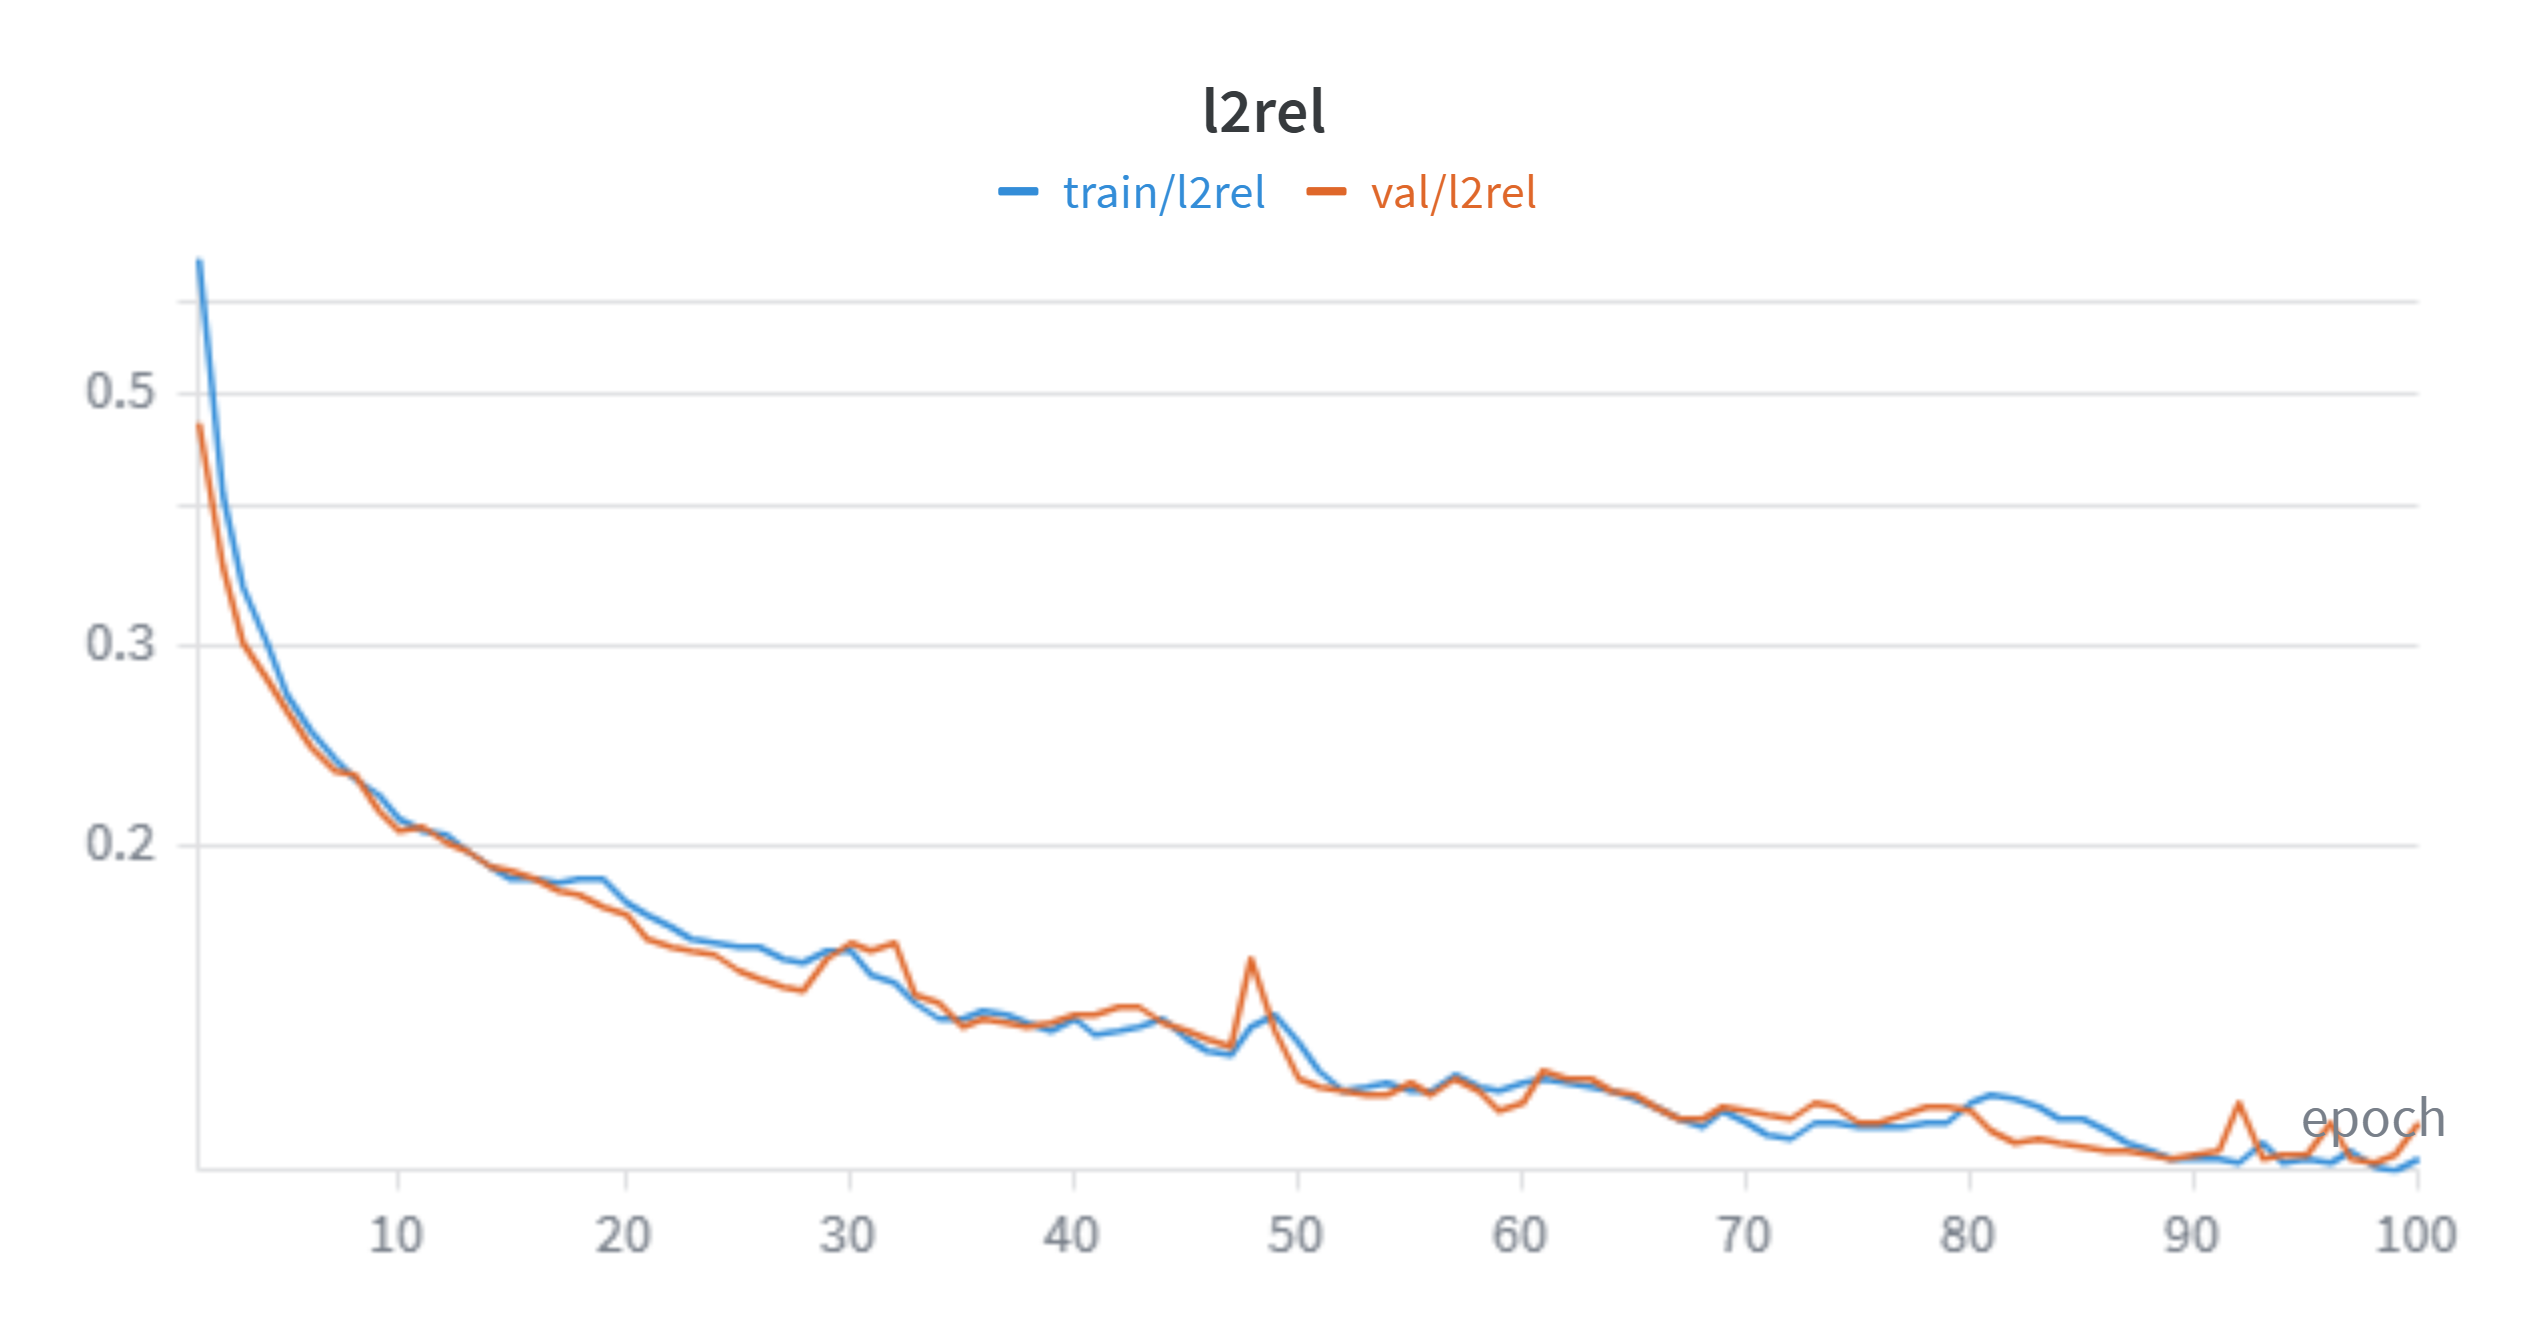
\includegraphics[height=3.8cm]{LaplaceAE_l2rel.png}
          \caption{Laplace AE L2 relative error}
      \end{figure}
      \column{0.5\textwidth}
      \begin{figure}
          \centering
          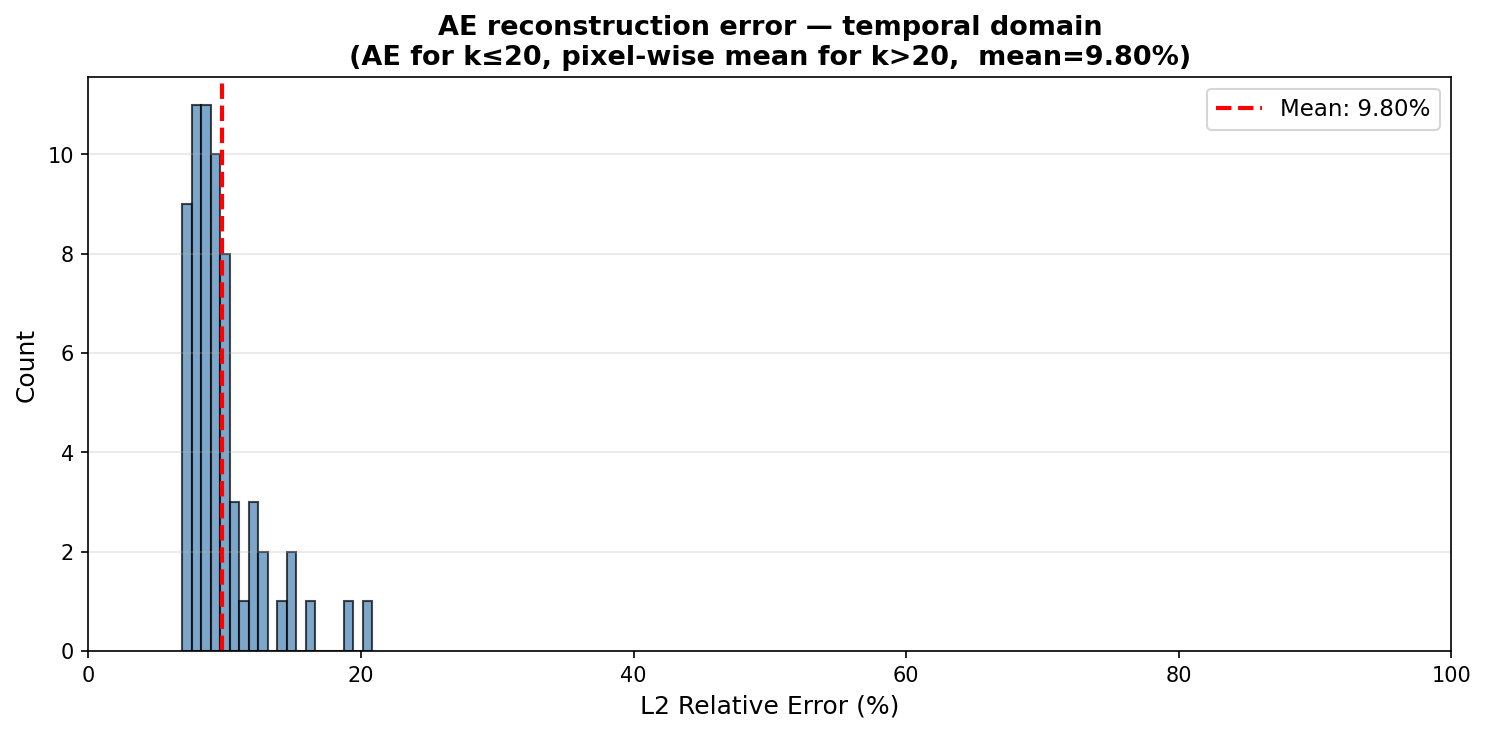
\includegraphics[height=3.8cm]{ae_study_temporal_error.png}
          \caption{Temporal error}
      \end{figure}
  \end{columns}
\end{frame}

\begin{frame}{Latent Space: Performance Evaluation per Frequency Index}
  Reconstruction error naturally degrades as we evaluate higher conditioning indices $k$. The model efficiently reconstructs the highly energetic low frequencies, while struggling with the noise-like high-frequency tail.
  \vspace{0.5em}
  \begin{figure}
      \centering
      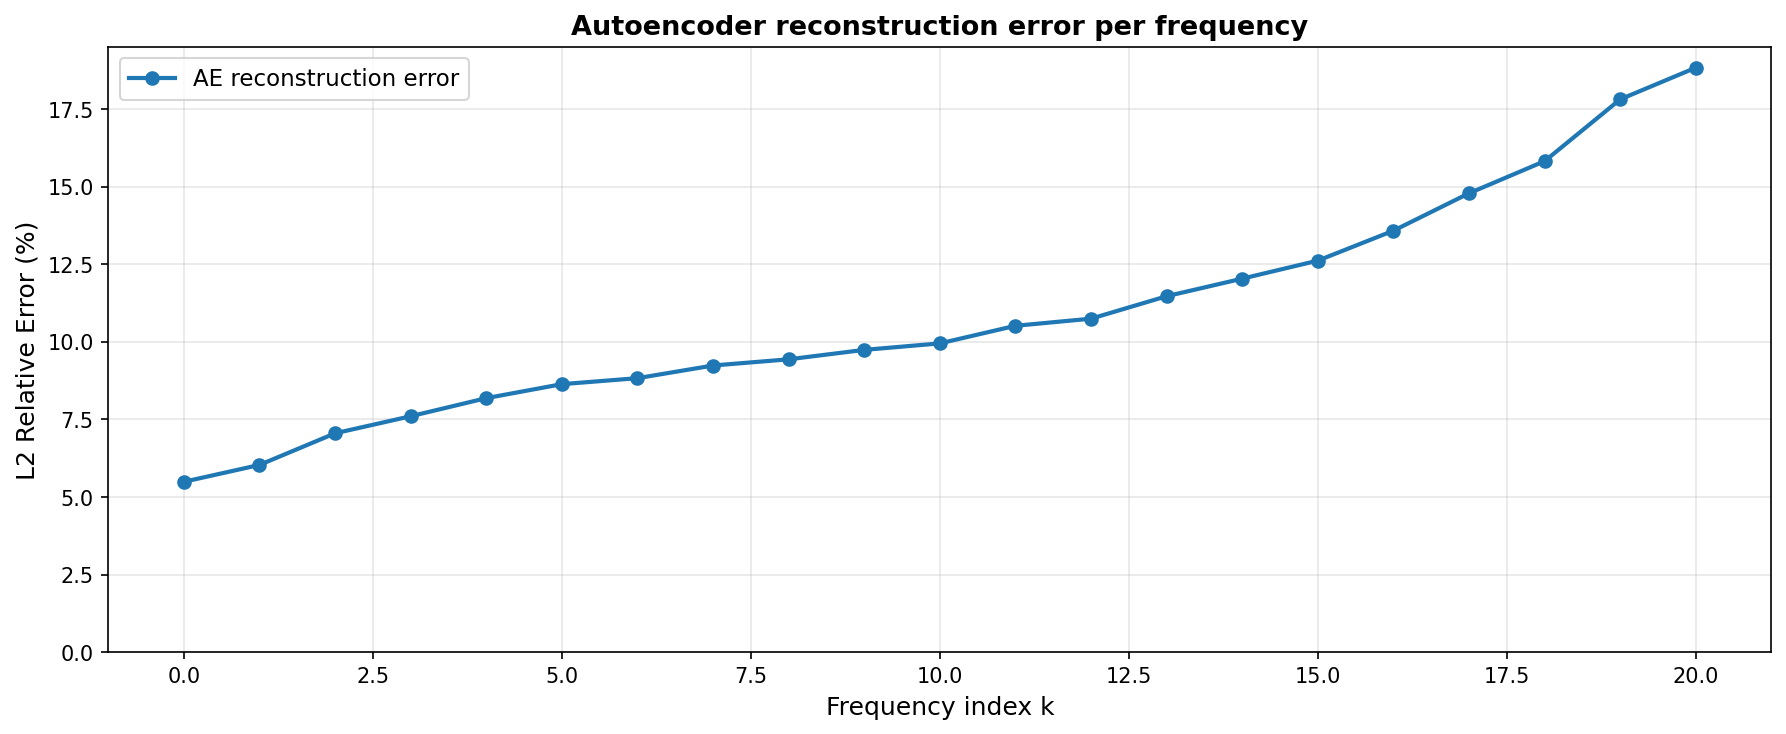
\includegraphics[height=5.5cm]{ae_study_frequency_error.png}
      \caption{AE Frequency error}
  \end{figure}
\end{frame}

\begin{frame}{Latent Space: Spatial Truncation Error per Frequency}
  Loss increases monotonically with frequency (up to 17\% at $k=20$). Low frequencies ($k=0$) feature smooth gradients; high frequencies ($k=20$) show widely distributed, highly oscillatory patterns.\\
  \vspace{1em}
  \begin{columns}
      \column{0.5\textwidth}
      \begin{figure}
          \centering
          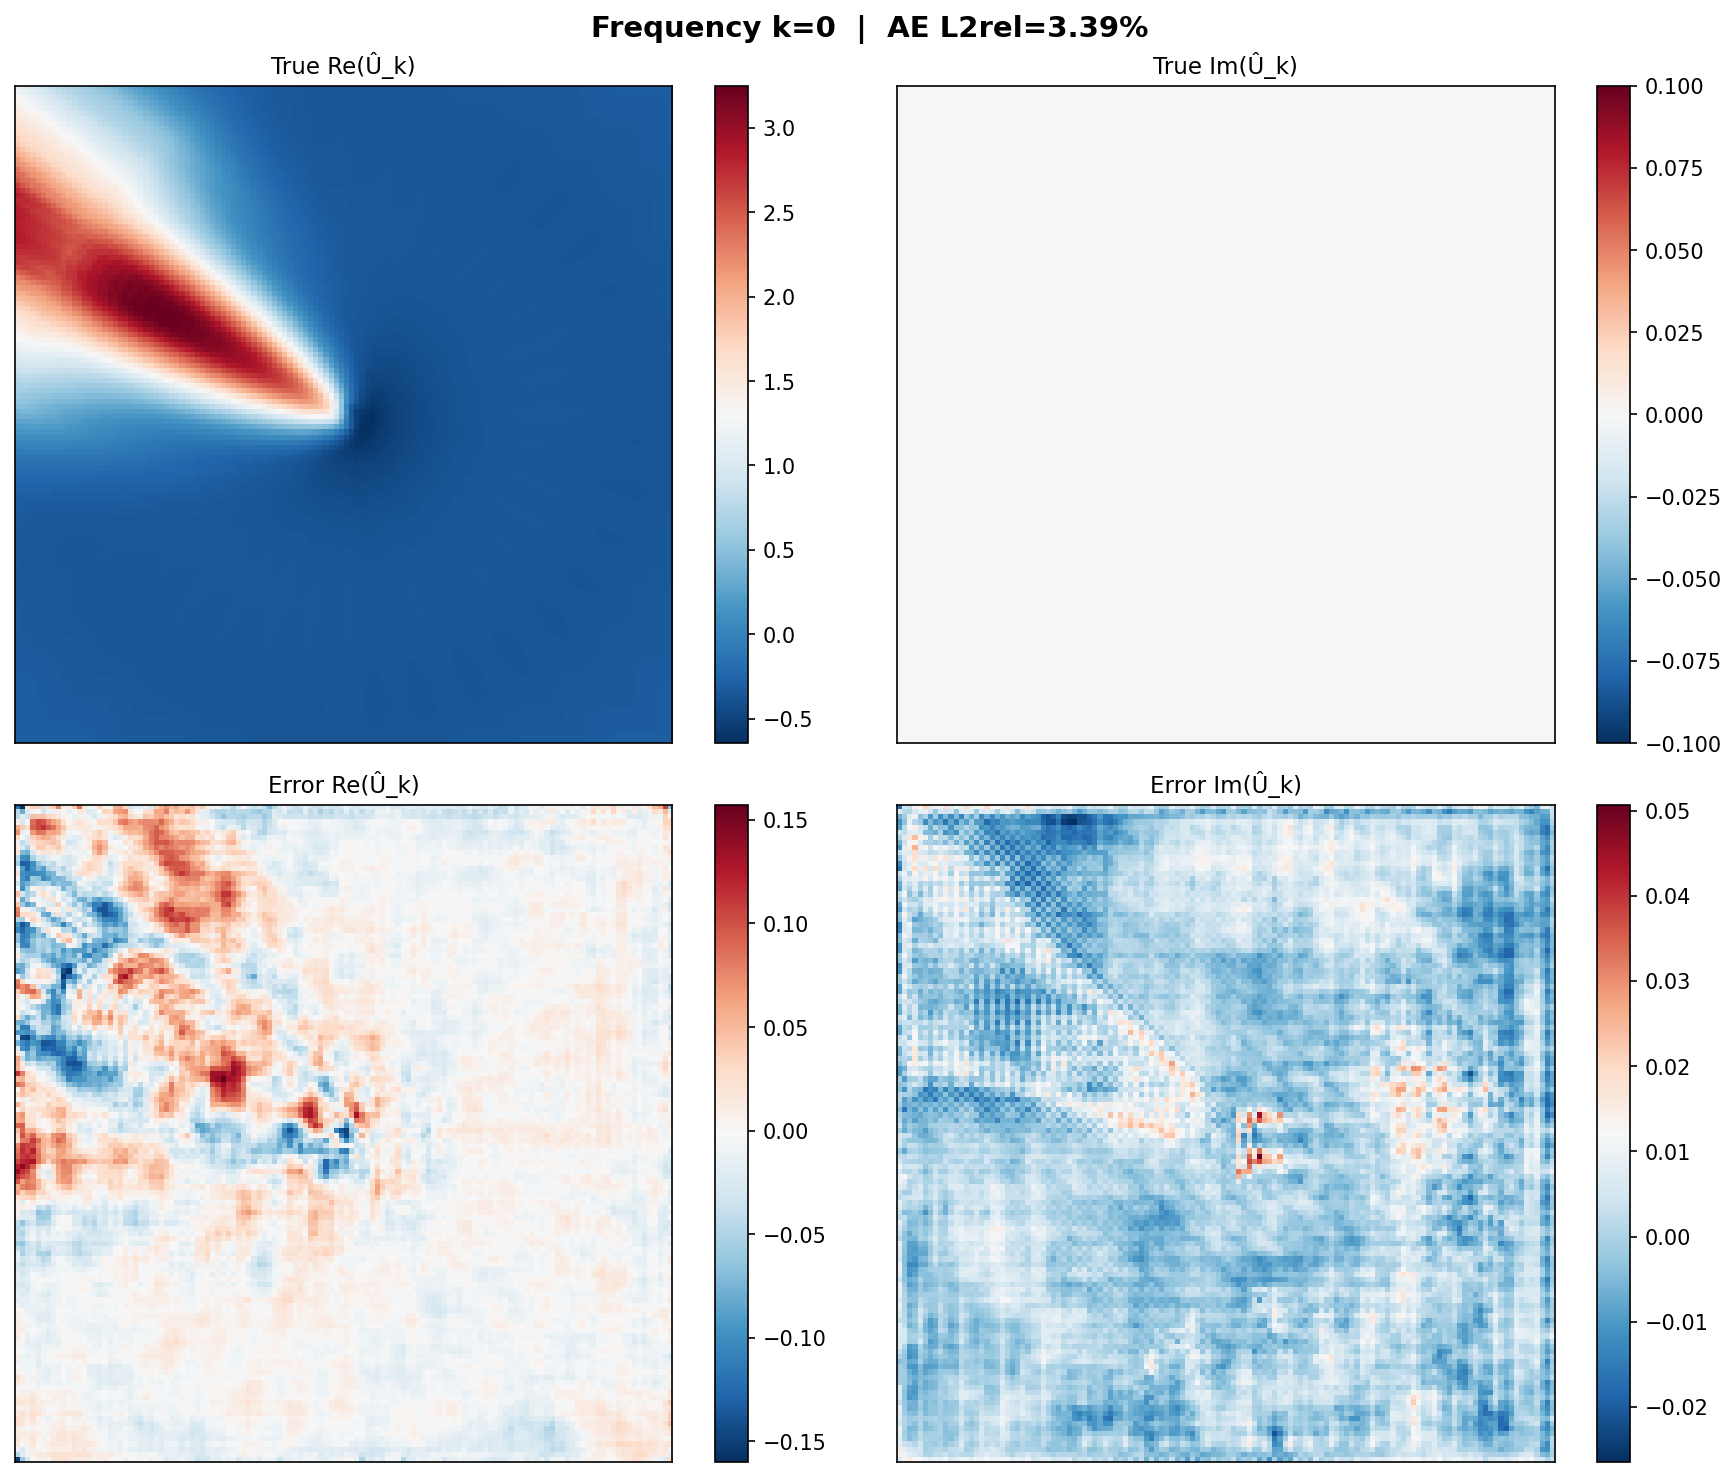
\includegraphics[height=4.5cm]{ae_study_freq_00.png}
          \caption{Spatial truncation at $k=0$ (DC)}
      \end{figure}
      \column{0.5\textwidth}
      \begin{figure}
          \centering
          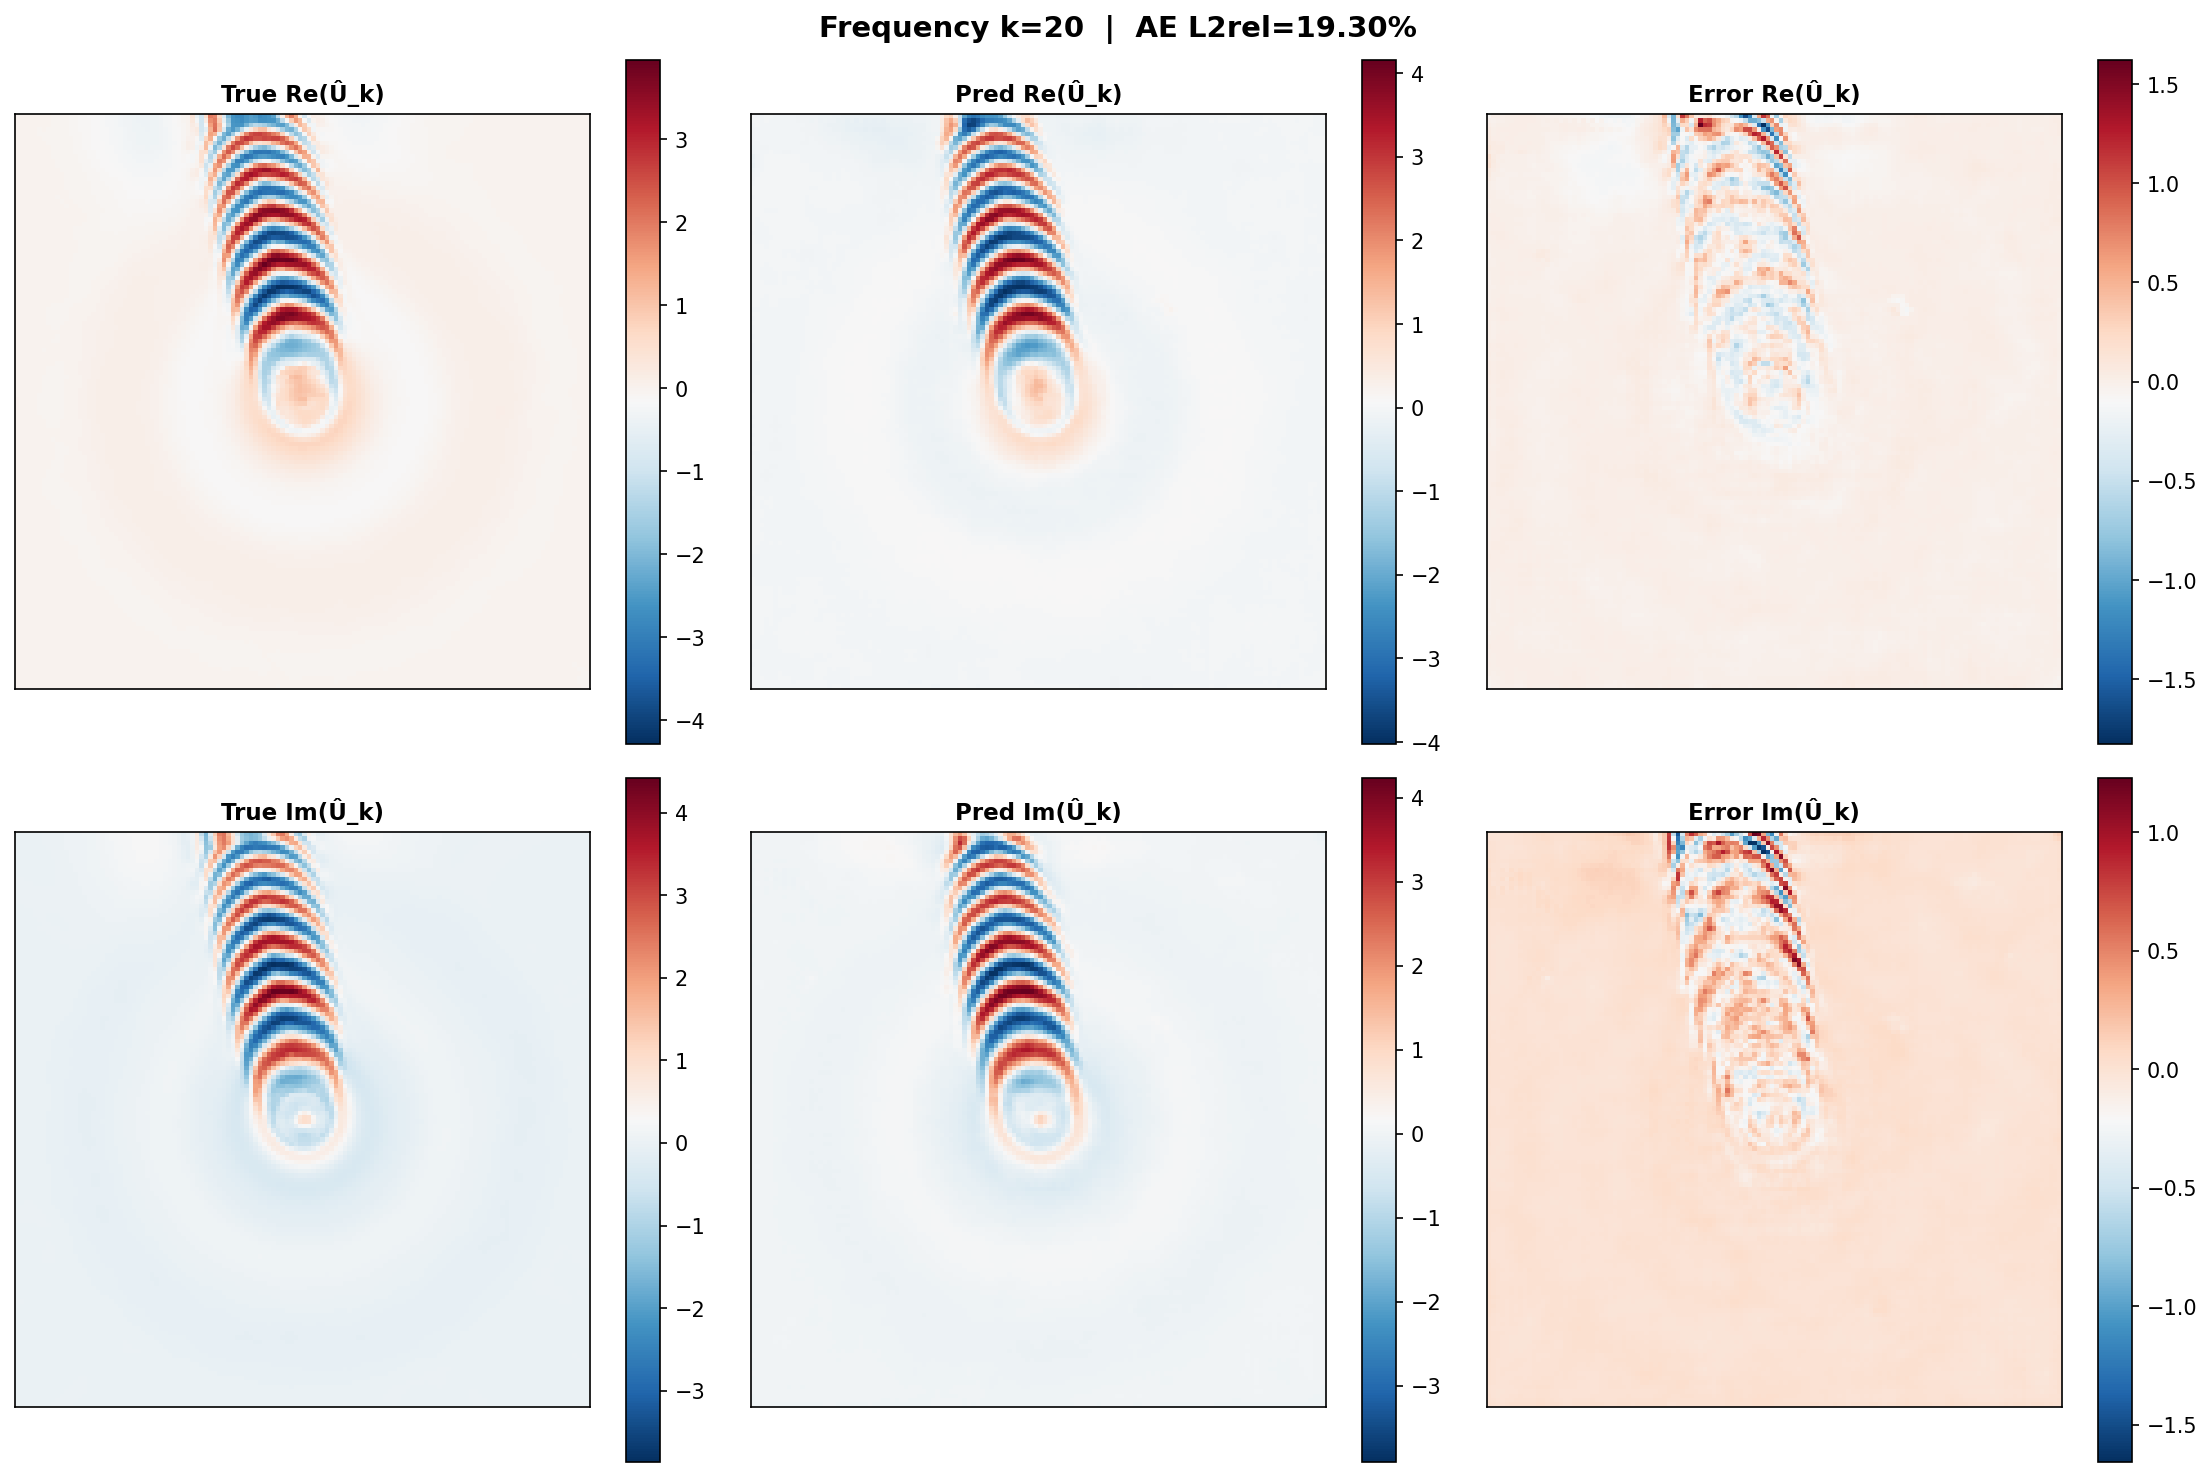
\includegraphics[height=4.5cm]{ae_study_freq_20.png}
          \caption{Spatial truncation at $k=20$ (High)}
      \end{figure}
  \end{columns}
\end{frame}

\begin{frame}{Demonstration: Latent Space Autoencoder}
  \textbf{Autoencoder Reconstruction over time}\\
  \vspace{0.5em}
  \begin{figure}
      \centering
      \animategraphics[loop,autoplay,width=0.8\textwidth]{10}{frames_ae_study_anim_0/frame_}{0}{149}
      \caption{Autoencoder reconstruction over time}
  \end{figure}
  \vspace{1em}
  \textit{The AE cleanly decodes the temporal trajectory when provided with true frequencies.}
\end{frame}


\begin{frame}{Phase 1: Frozen Latent Surrogates ($\vtheta \to z_k$)}
  21 Independent MLPs (one per frequency) directly regress parameter $\vtheta$ into precomputed $z_k$.\\
  \textbf{Observe the Sawtooth dynamics}: High frequencies are increasingly difficult to predict.
  
  \vspace{0.5em}
  \begin{columns}
      \column{0.5\textwidth}
      \begin{figure}
          \centering
          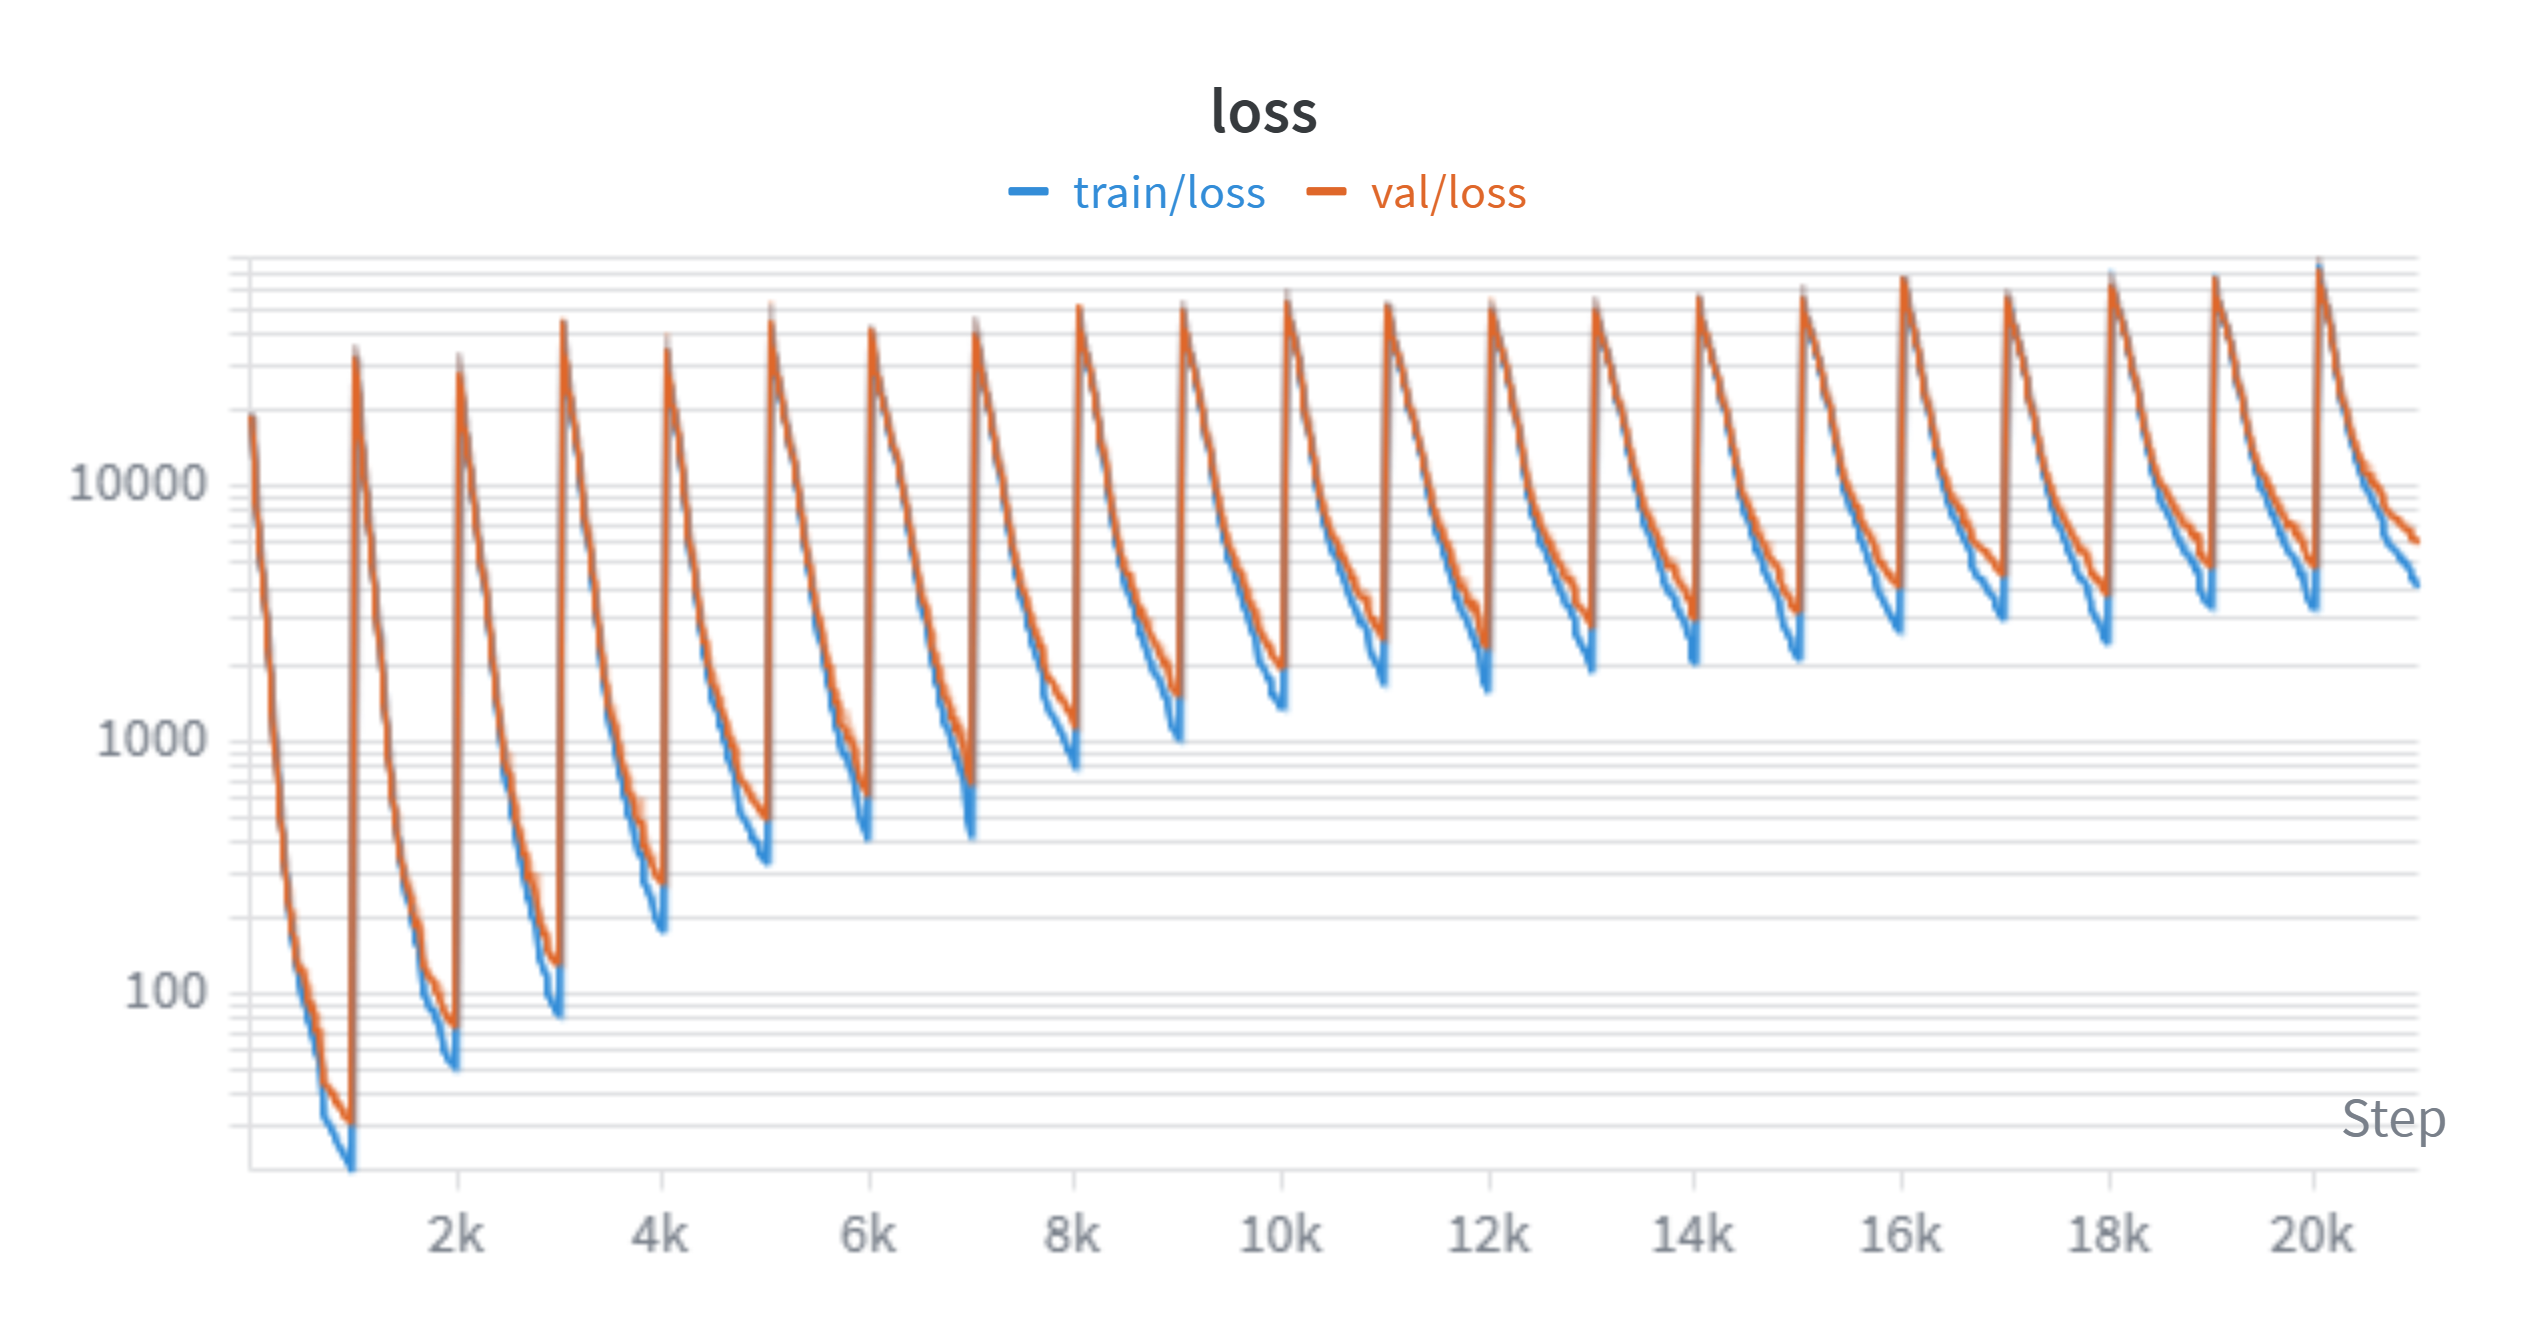
\includegraphics[height=3.8cm]{LaplaceLatentSurrogate_Nt150_loss.png}
          \caption{Latent surrogate loss}
      \end{figure}
      \column{0.5\textwidth}
      \begin{figure}
          \centering
          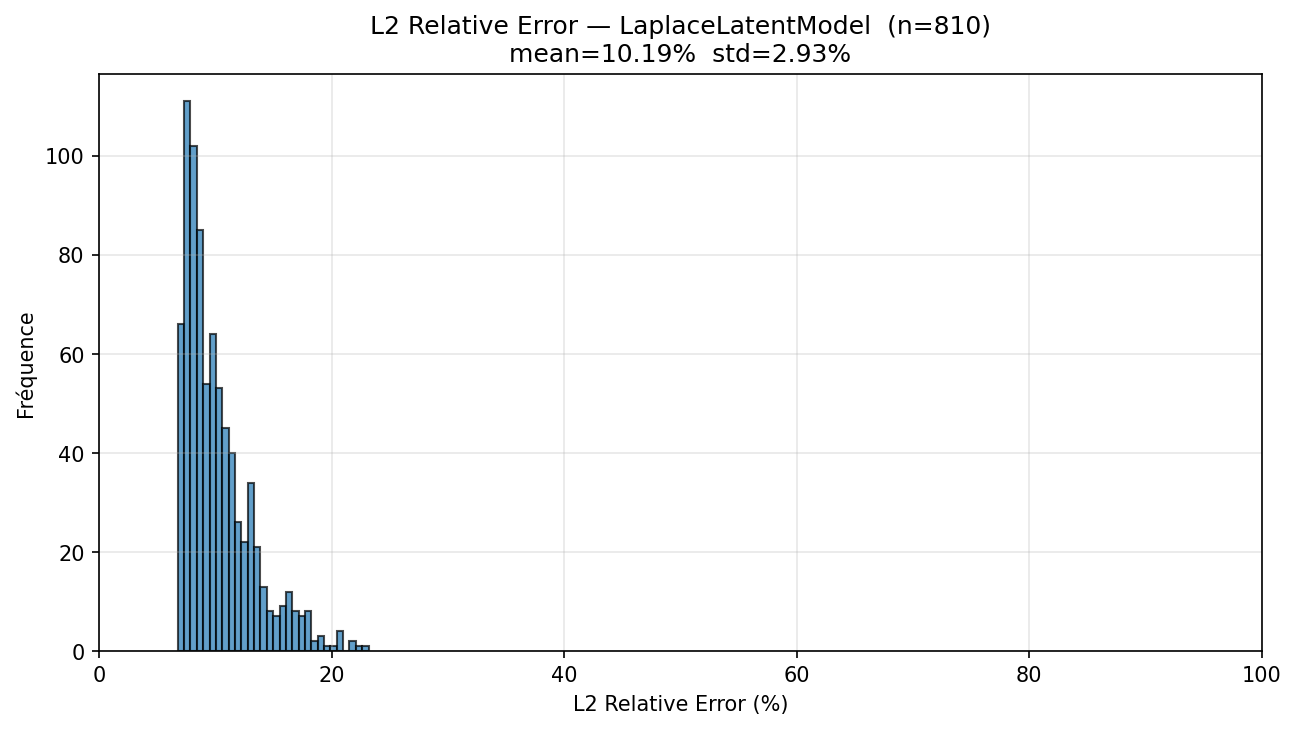
\includegraphics[height=3.8cm]{laplacelatentmodel_l2rel_hist.png}
          \caption{Latent surrogate relative error}
      \end{figure}
  \end{columns}
\end{frame}

\begin{frame}{Phase 2: End-to-End Fine-Tuning}
  We unfreeze the AE Decoder and train the whole physical map end-to-end through the differentiable Laplace inversion. This directly minimises physical error, \textbf{halving the median error (9.30\%)}.
  
  \vspace{0.5em}
  \begin{columns}
      \column{0.5\textwidth}
      \begin{figure}
          \centering
          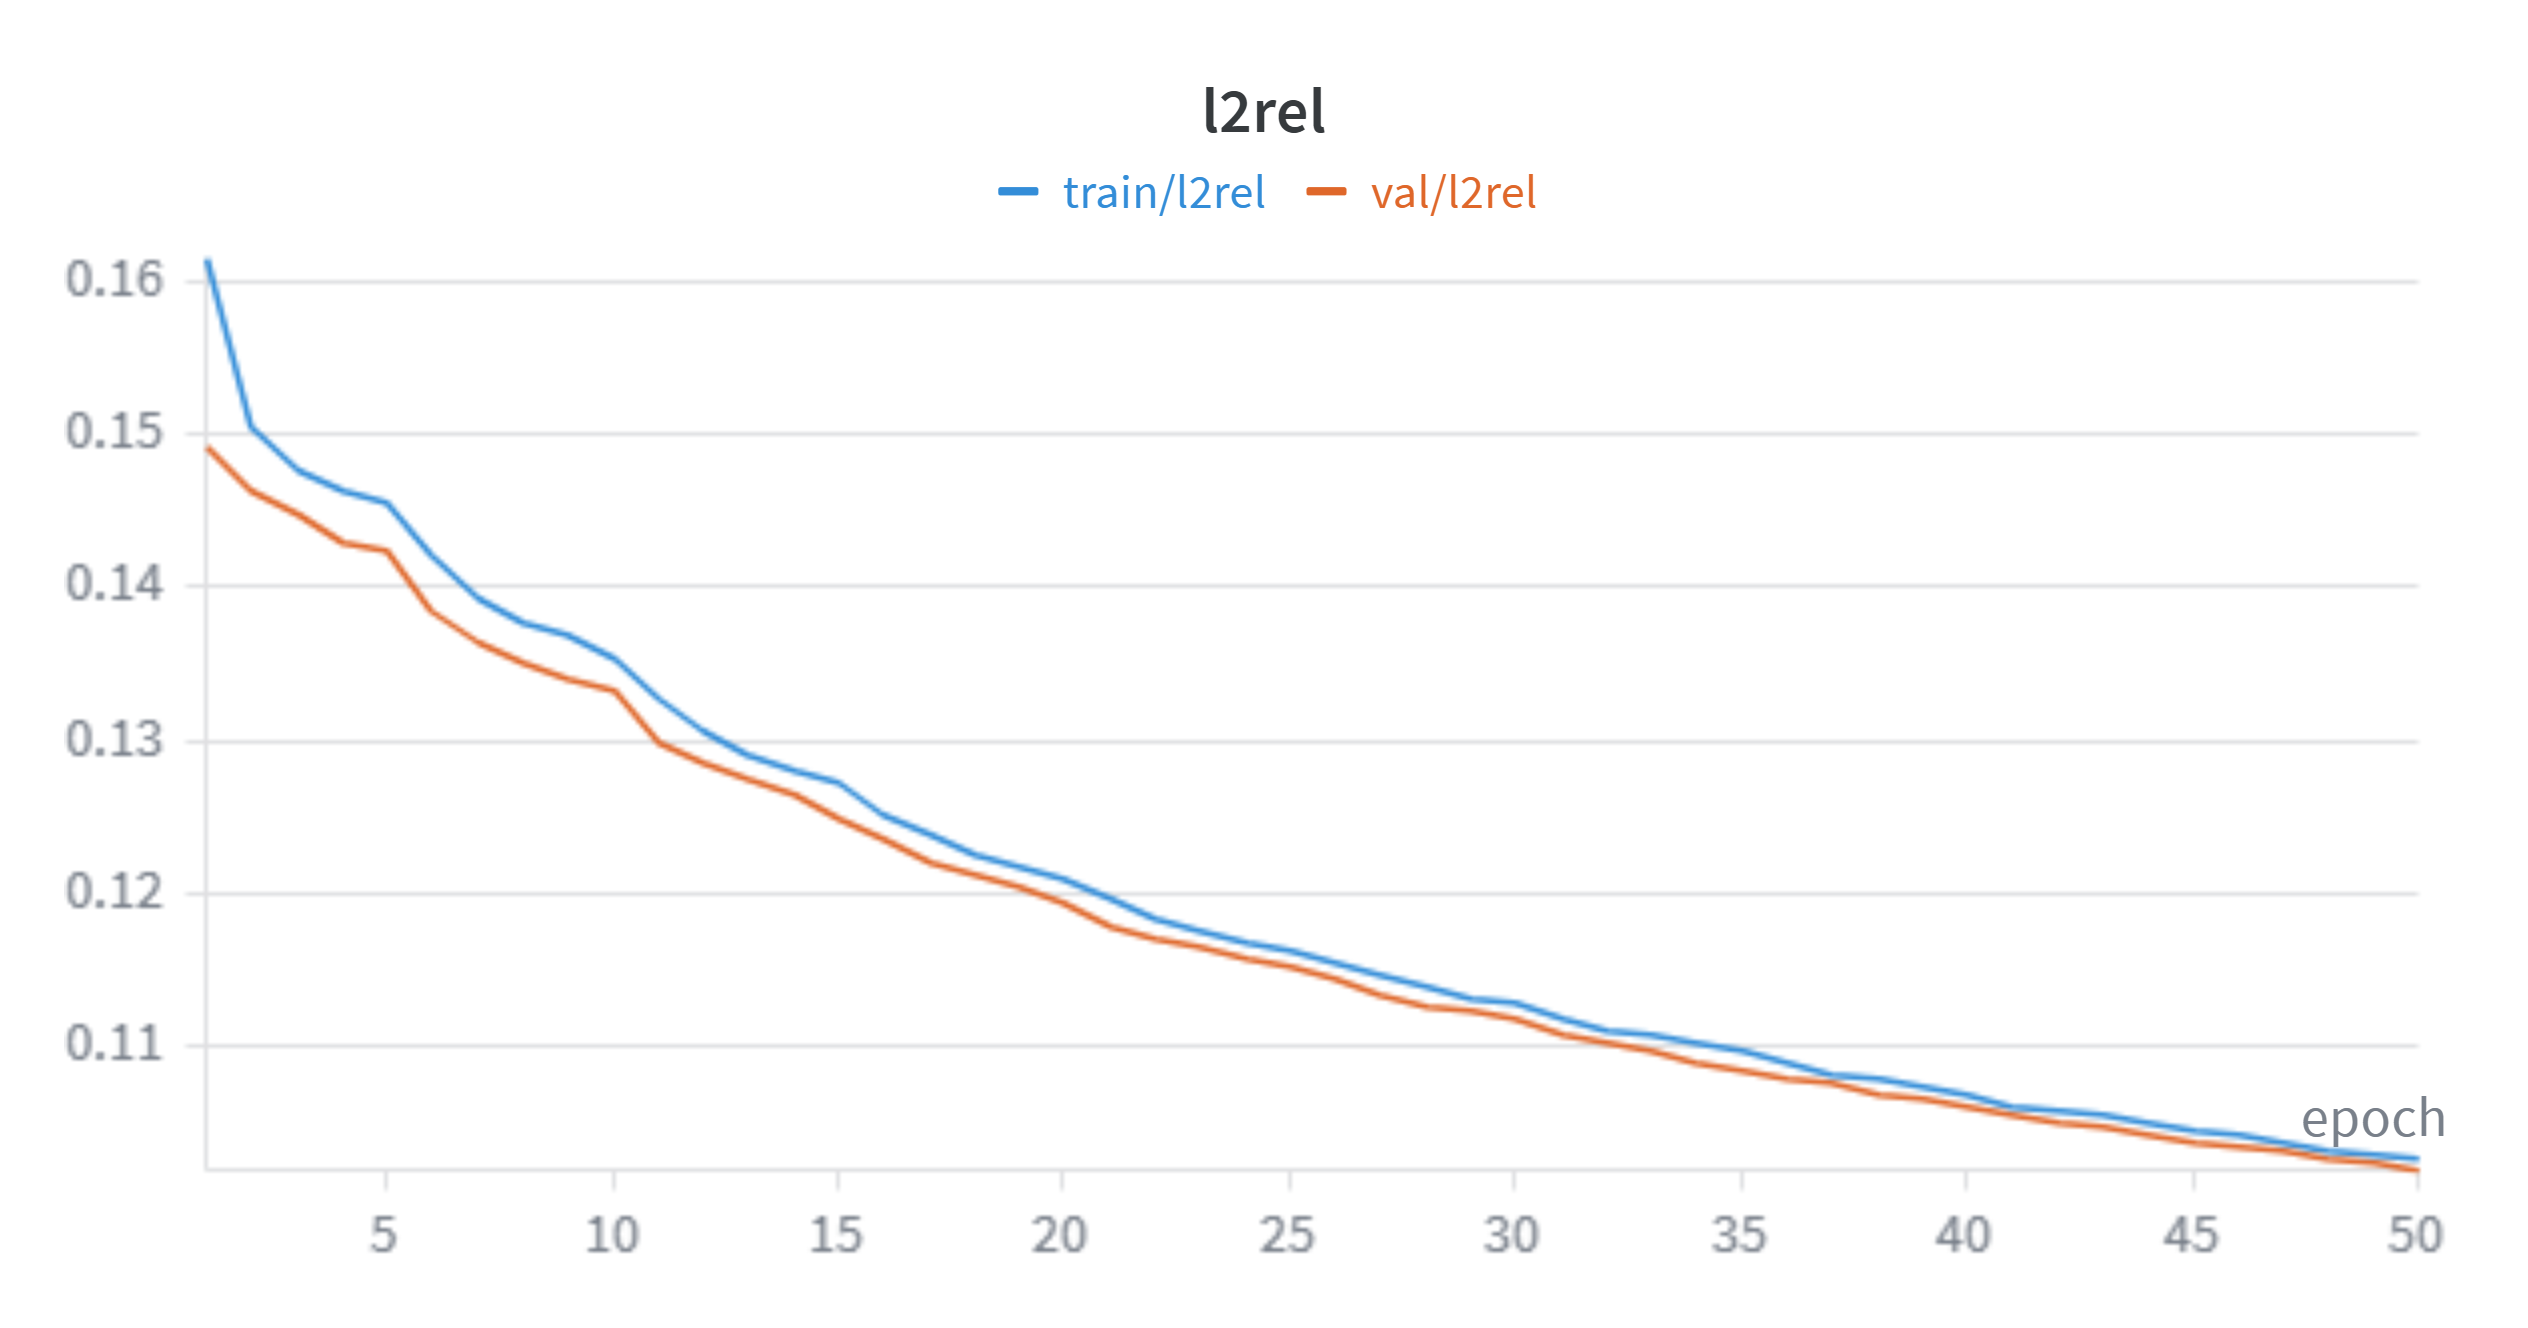
\includegraphics[height=3.8cm]{LaplaceLatentModel_finetune_e2e.png}
          \caption{E2E fine-tuning loss}
      \end{figure}
      \column{0.5\textwidth}
      \begin{figure}
          \centering
          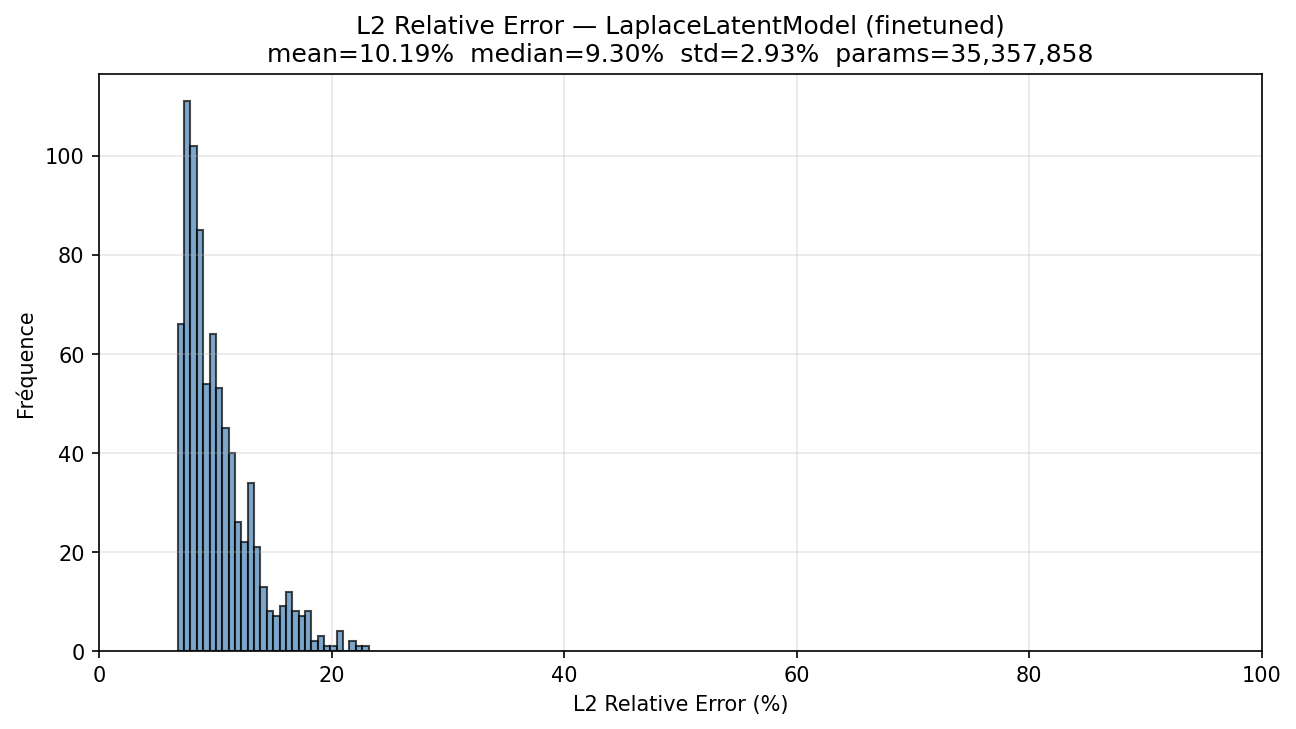
\includegraphics[height=3.8cm]{laplacelatentmodel_finetuned_l2rel_hist.png}
          \caption{Fine-tuned physical map error}
      \end{figure}
  \end{columns}
\end{frame}

\begin{frame}{Demonstration: Fine-Tuned Physical Map}
  \textbf{End-to-End Surrogate Emulation}\\
  \vspace{0.5em}
  \begin{figure}
      \centering
      \animategraphics[loop,autoplay,width=0.8\textwidth]{10}{frames_LaplaceLatentModel_anim_1/frame_}{0}{149}
      \caption{End-to-End surrogate emulation}
  \end{figure}
  \vspace{1em}
  \textit{After fine-tuning, the surrogate successfully bridges the parameters to the non-linear transport dynamics.}
\end{frame}

\begin{frame}{Phase 3: Residual Corrector (Gibbs Phenomenon)}
  Spectral truncation at $k_{\max}=20$ creates inherent ripples. A 3D UNet (+481k params) suppresses ripples frame-by-frame on frozen surrogate predictions, reducing error to \textbf{4.46\%}.
  
  \vspace{0.5em}
  \begin{columns}
      \column{0.5\textwidth}
      \begin{figure}
          \centering
          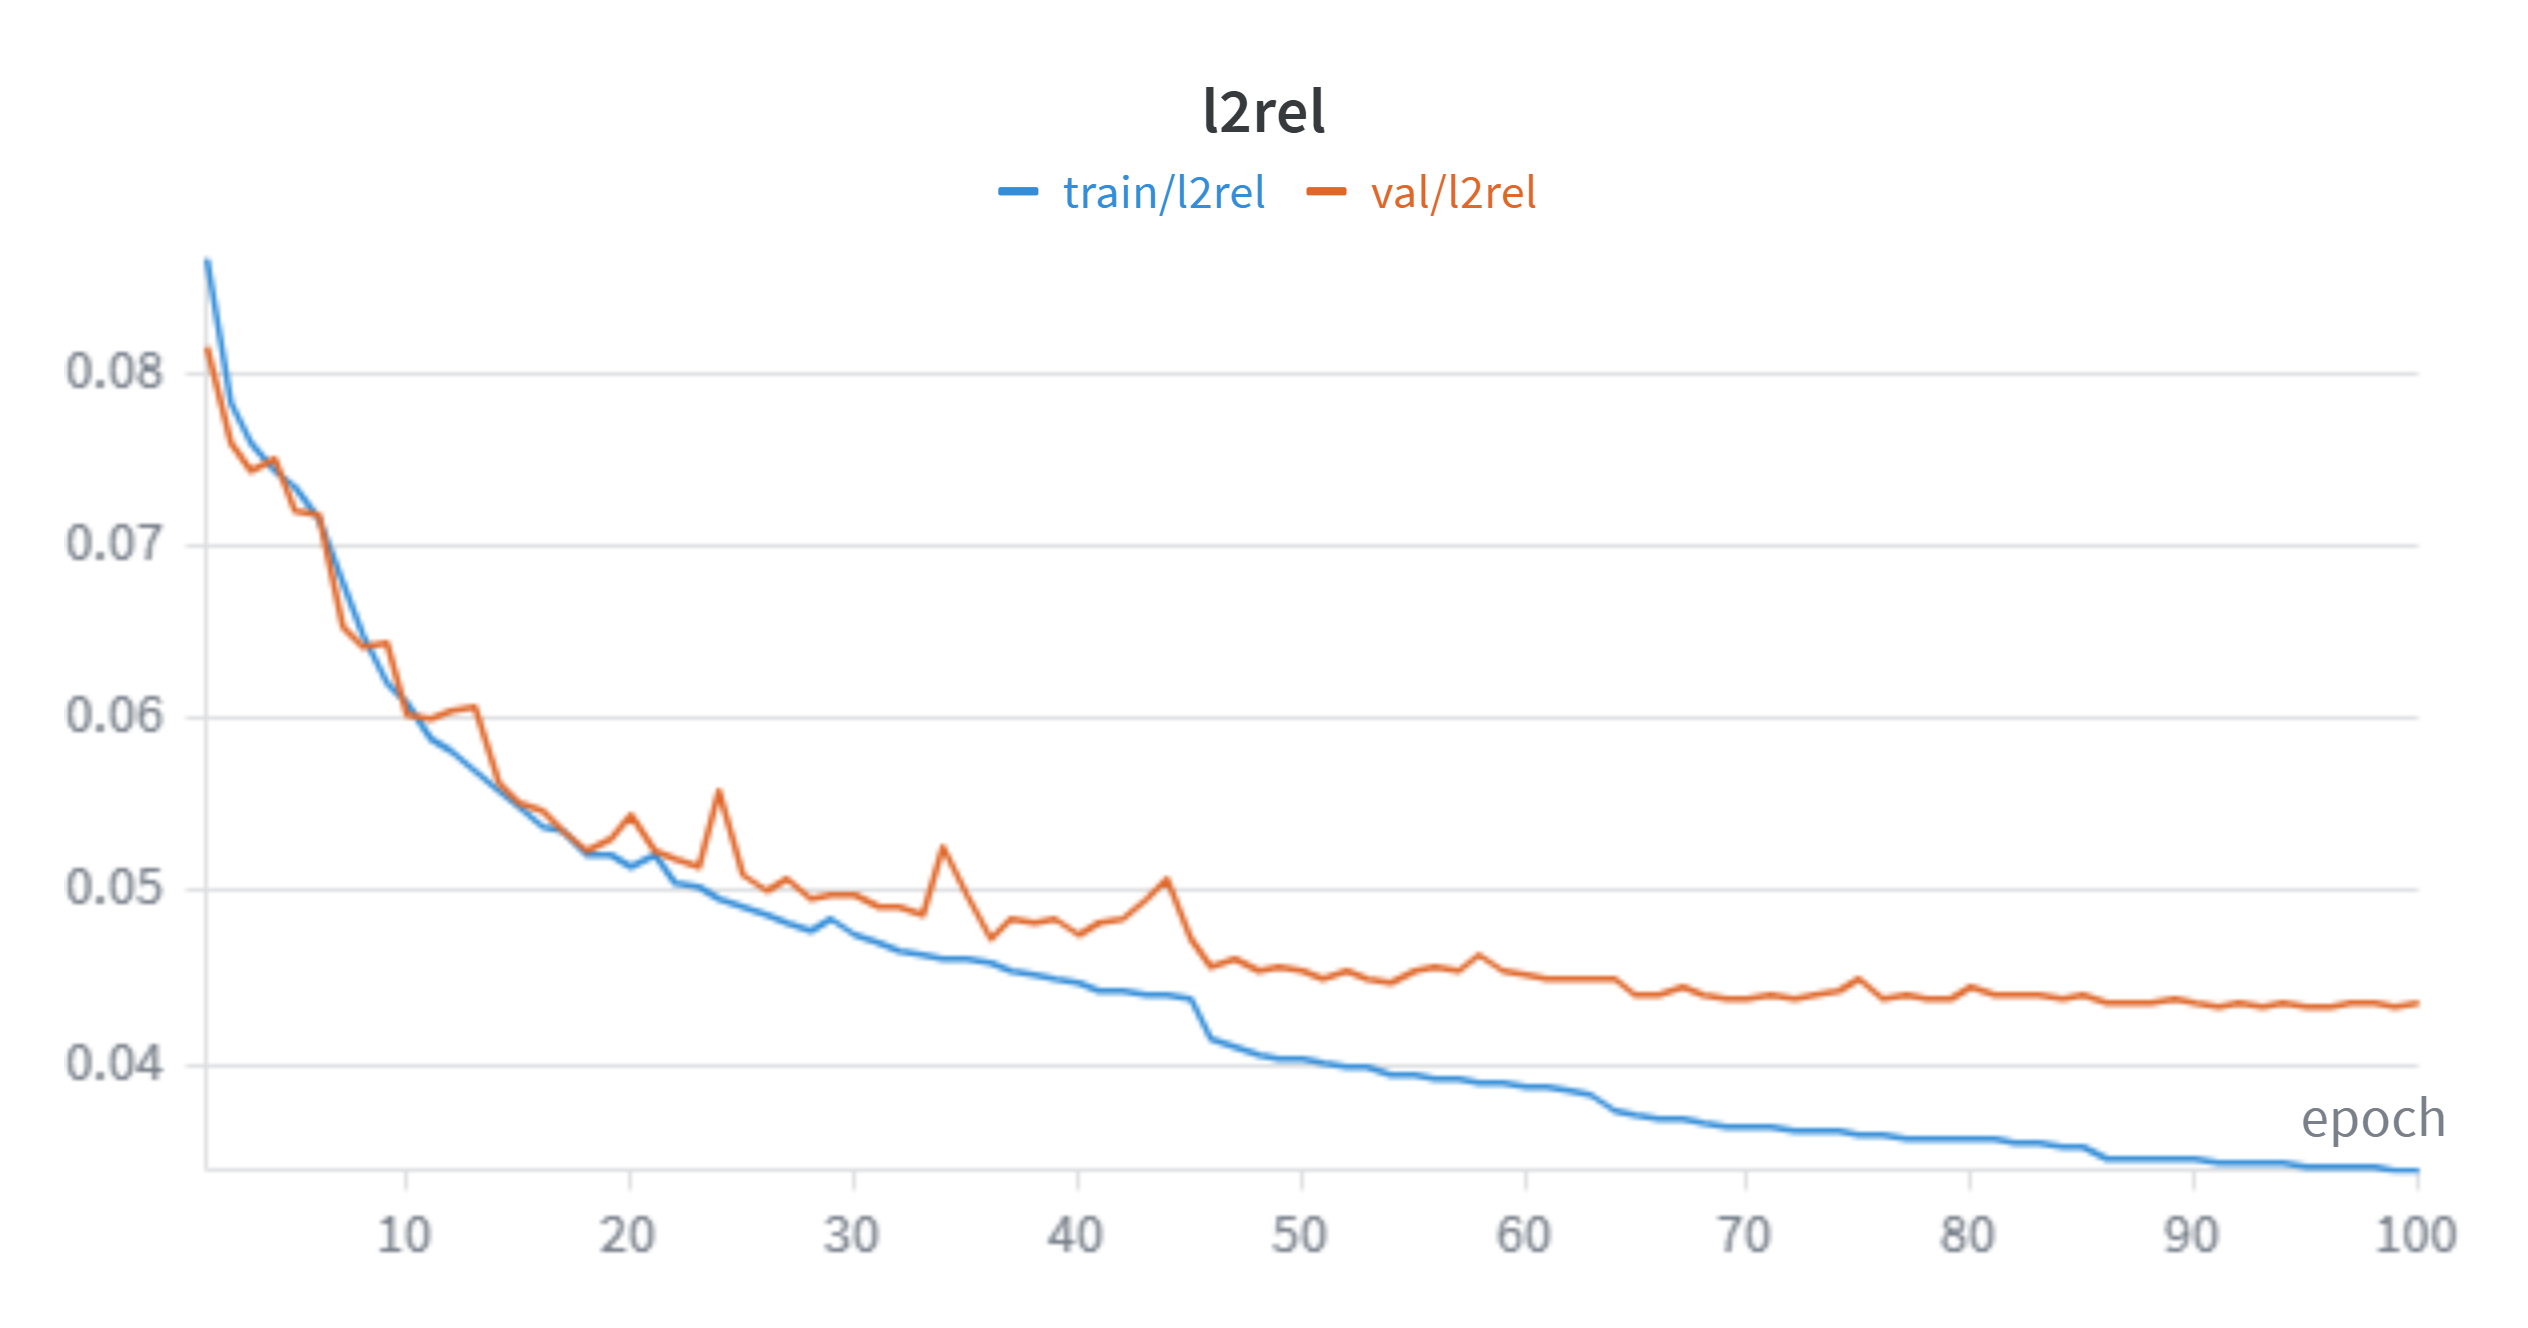
\includegraphics[height=3.8cm]{CorrectionAE_l2rel.png}
          \caption{Residual Corrector error over time}
      \end{figure}
      \column{0.5\textwidth}
      \begin{figure}
          \centering
          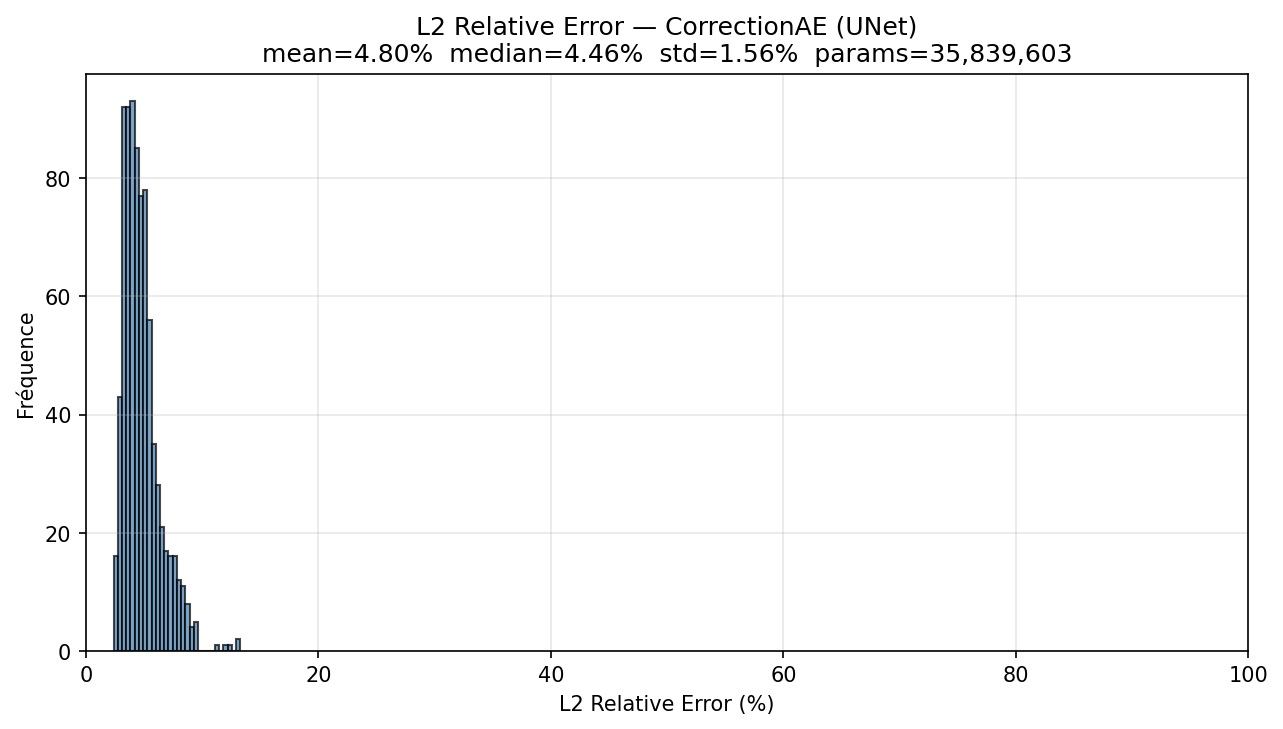
\includegraphics[height=3.8cm]{correctionae_unet_l2rel_hist.png}
          \caption{Residual Corrector relative error}
      \end{figure}
  \end{columns}
\end{frame}

\begin{frame}{Demonstration: Residual Corrector}
  \textbf{Post-Hoc Gibbs Artifact Suppression}\\
  \vspace{0.5em}
  \begin{figure}
      \centering
      \animategraphics[loop,autoplay,width=0.8\textwidth]{10}{frames_CorrectionAE_anim_1/frame_}{0}{149}
      \caption{Gibbs artifact suppression}
  \end{figure}
  \vspace{1em}
  \textit{The 3D UNet effectively suppresses spatial ripples dynamically over time.}
\end{frame}

\begin{frame}{Inference Pipeline Architecture}
\definecolor{clrA}{RGB}{224,233,245}
\definecolor{clrB}{RGB}{200,218,240}
\definecolor{clrC}{RGB}{208,226,234}
\definecolor{clrD}{RGB}{246,228,202}
\definecolor{clrE}{RGB}{232,220,242}
\definecolor{clrF}{RGB}{210,235,215}
\definecolor{bdrA}{RGB}{95,135,185}
\definecolor{bdrB}{RGB}{65,115,170}
\definecolor{bdrC}{RGB}{55,125,155}
\definecolor{bdrD}{RGB}{185,135,55}
\definecolor{bdrE}{RGB}{125,85,165}
\definecolor{bdrF}{RGB}{65,140,85}
\begin{figure}
\centering
\resizebox{0.95\textwidth}{!}{%
\begin{tikzpicture}[
  >=Stealth,
  rbox/.style={rectangle, rounded corners=2pt,
    text width=3.1cm, minimum height=1.7cm,
    align=center, inner sep=6pt, font=\sffamily\footnotesize},
  sbox/.style={rectangle, rounded corners=2pt,
    text width=2.1cm, minimum height=0.85cm,
    align=center, inner sep=3pt, font=\sffamily\scriptsize},
  arr/.style={-Stealth, line width=0.65pt, black!40},
]

%% ── INPUT (includes normalisation) ──────────────────────────
\node[rbox, draw=bdrA, fill=clrA] (input) at (0, 0) {
  \textbf{Input}\\[2pt]
  $\vtheta_{\mathrm{raw}}=(k,\,A,\,C)$\\
  {\sffamily\scriptsize $\vtheta_{\mathrm{norm}}=(\vtheta_{\mathrm{raw}}-\mu_{\vtheta})/\sigma_{\vtheta}$}\\[3pt]
  {\sffamily\scriptsize\itshape\color{black!35} $(B,\,3)$}
};

%% ── PARALLEL MLPs ────────────────────────────────────────────
\node[sbox, draw=bdrB, fill=clrB] (mlp0)  at (5.2,  1.5) {
  $\mathrm{proj}_0:\vtheta_{\mathrm{norm}}\!\to\!z_0$\\[2pt]
  {\sffamily\tiny\color{black!35} $z_0:(B,\,64)$}
};
\node[sbox, draw=bdrB, fill=clrB] (mlpk)  at (5.2,  0.3) {
  $\mathrm{proj}_k:\vtheta_{\mathrm{norm}}\!\to\!z_k$\\[2pt]
  {\sffamily\tiny\color{black!35} $z_k:(B,\,64)$}
};
\node[font=\normalsize\sffamily, text=black!45] (vdots) at (5.2, -0.5) {$\vdots$};
\node[sbox, draw=bdrB, fill=clrB] (mlp20) at (5.2, -1.2) {
  $\mathrm{proj}_{20}:\vtheta_{\mathrm{norm}}\!\to\!z_{20}$\\[2pt]
  {\sffamily\tiny\color{black!35} $z_{20}:(B,\,64)$}
};
% architecture note shared across all
\node[font=\sffamily\tiny, text=black!40, align=center] at (5.2, -1.9)
  {$3\!\to\!128\!\to\!256^2\!\to\!64$, LN+ReLU};

% dashed enclosure
\node[draw=bdrB, dashed, rounded corners=3pt, line width=0.5pt,
      fit=(mlp0)(mlp20)(vdots),
      inner sep=8pt,
      label={[font=\sffamily\scriptsize, text=bdrB, inner sep=2pt]above:
             \textit{21 independent surrogates (one per frequency)}}] (mlpgroup) {};

%% ── CONCAT + FREQ RATIOS ─────────────────────────────────────
\node[rbox, draw=bdrB, fill=clrB] (concat) at (10.5, 0) {
  \textbf{Concat + freq.\ ratios}\\[2pt]
  $[z_0,\ldots,z_{20}]$\\
  $f_k = k/(N_{\mathrm{half}}-1)$\\[3pt]
  {\sffamily\scriptsize\itshape\color{black!35} $(21B,\,64)$}
};

%% ── SHARED DECODER ───────────────────────────────────────────
\node[rbox, draw=bdrC, fill=clrC] (decoder) at (15.2, 0) {
  \textbf{Shared Decoder}\\
  {\sffamily\scriptsize FiLM on $f_k$}\\[2pt]
  {\sffamily\scriptsize FC\;$\to$\;3$\times$ConvT\;$\to$\;Re/Im}\\[2pt]
  {\sffamily\scriptsize\itshape\color{black!35} $(B,\,21,\,2,\,N,\!N)$}
};

%% ── ROW 2: right → left ──────────────────────────────────────
\node[rbox, draw=bdrD, fill=clrD] (denorm) at (15.2, -4.0) {
  \textbf{Denorm + spectrum}\\[2pt]
  $k>k_{\max}$: $\tilde{U}_k\leftarrow\bar{U}^{(k)}$\\
  $\tilde{U}_{N_t-k}:=\overline{\tilde{U}_k}$\\[2pt]
  {\sffamily\scriptsize\itshape\color{black!35} $(B,\,N^2,\,150)_{\mathbb{C}}$}
};
\node[rbox, draw=bdrD, fill=clrD] (ifft) at (10.5, -4.0) {
  \textbf{Inverse Laplace}\\[2pt]
  $U_{\mathrm{surr}}=\mathrm{Re}[\mathrm{IFFT}(\tilde{U})]$\\
  $/\,(dt\!\cdot\!w_t\!\cdot\!e^{-\gamma t})$\\[2pt]
  {\sffamily\scriptsize\itshape\color{black!35} $(B,\,150,\,N,\!N)$}
};
\node[rbox, draw=bdrE, fill=clrE] (unet) at (5.2, -4.0) {
  \textbf{Residual UNet}\\[2pt]
  $U_{\mathrm{corr}}=U_{\mathrm{surr}}+\sigma r\!\bigl(\tfrac{U_{\mathrm{surr}}-\mu}{\sigma}\bigr)$\\
  {\sffamily\scriptsize 3-level enc./dec.\ + skip}\\[2pt]
  {\sffamily\scriptsize\itshape\color{black!35} $(B,\,150,\,N,\!N)$}
};
\node[rbox, draw=bdrF, fill=clrF] (output) at (0, -4.0) {
  \textbf{Output}\\[3pt]
  $U_{\mathrm{corr}}(t)$\\[2pt]
  {\sffamily\scriptsize CH$_4$ conc.\ field}\\[3pt]
  {\sffamily\scriptsize\itshape\color{black!35} $(B,\,150,\,128,\!128)$}
};

%% ── ARROWS ───────────────────────────────────────────────────
% Input → MLPs (fan out)
\draw[arr] (input.east) to[out=20,  in=180] (mlp0.west);
\draw[arr] (input.east) to[out=5,   in=180] (mlpk.west);
\draw[arr] (input.east) to[out=-15, in=180] (mlp20.west);

% MLPs → Concat (fan in)
\draw[arr] (mlp0.east)  to[out=0, in=150] (concat.west);
\draw[arr] (mlpk.east)  to[out=0, in=175] (concat.west);
\draw[arr] (mlp20.east) to[out=0, in=210] (concat.west);

% Main pipeline
\draw[arr] (concat.east)  -- (decoder.west);
\draw[arr] (decoder.south) -- (denorm.north);
\draw[arr] (denorm.west)  -- (ifft.east);
\draw[arr] (ifft.west)    -- (unet.east);
\draw[arr] (unet.west)    -- (output.east);

\end{tikzpicture}%
}
\caption{Inference Pipeline Architecture}
\end{figure}
\end{frame}

\section{Summary}

\begin{frame}{Complete Pipeline Benchmark Overview}
  \begin{table}
      \centering
      \scalebox{0.65}{
      \begin{tabular}{l c c c}
          \toprule
          \textbf{Method} & \textbf{Median} & \textbf{Std} & \textbf{Range} \\
          \midrule
          Baseline & 18.50\% & 5.35\% & 12.92 -- 48.80\% \\
          Finetuned E2E & \textbf{9.30\%} & 2.93\% & 6.75 -- 23.18\% \\
          \textbf{+ UNet Corr.} & \textbf{4.46\%} & \textbf{1.56\%} & \textbf{2.37 -- 13.28\%} \\
          \bottomrule
      \end{tabular}}
  \end{table}
  
  \begin{figure}
      \centering
      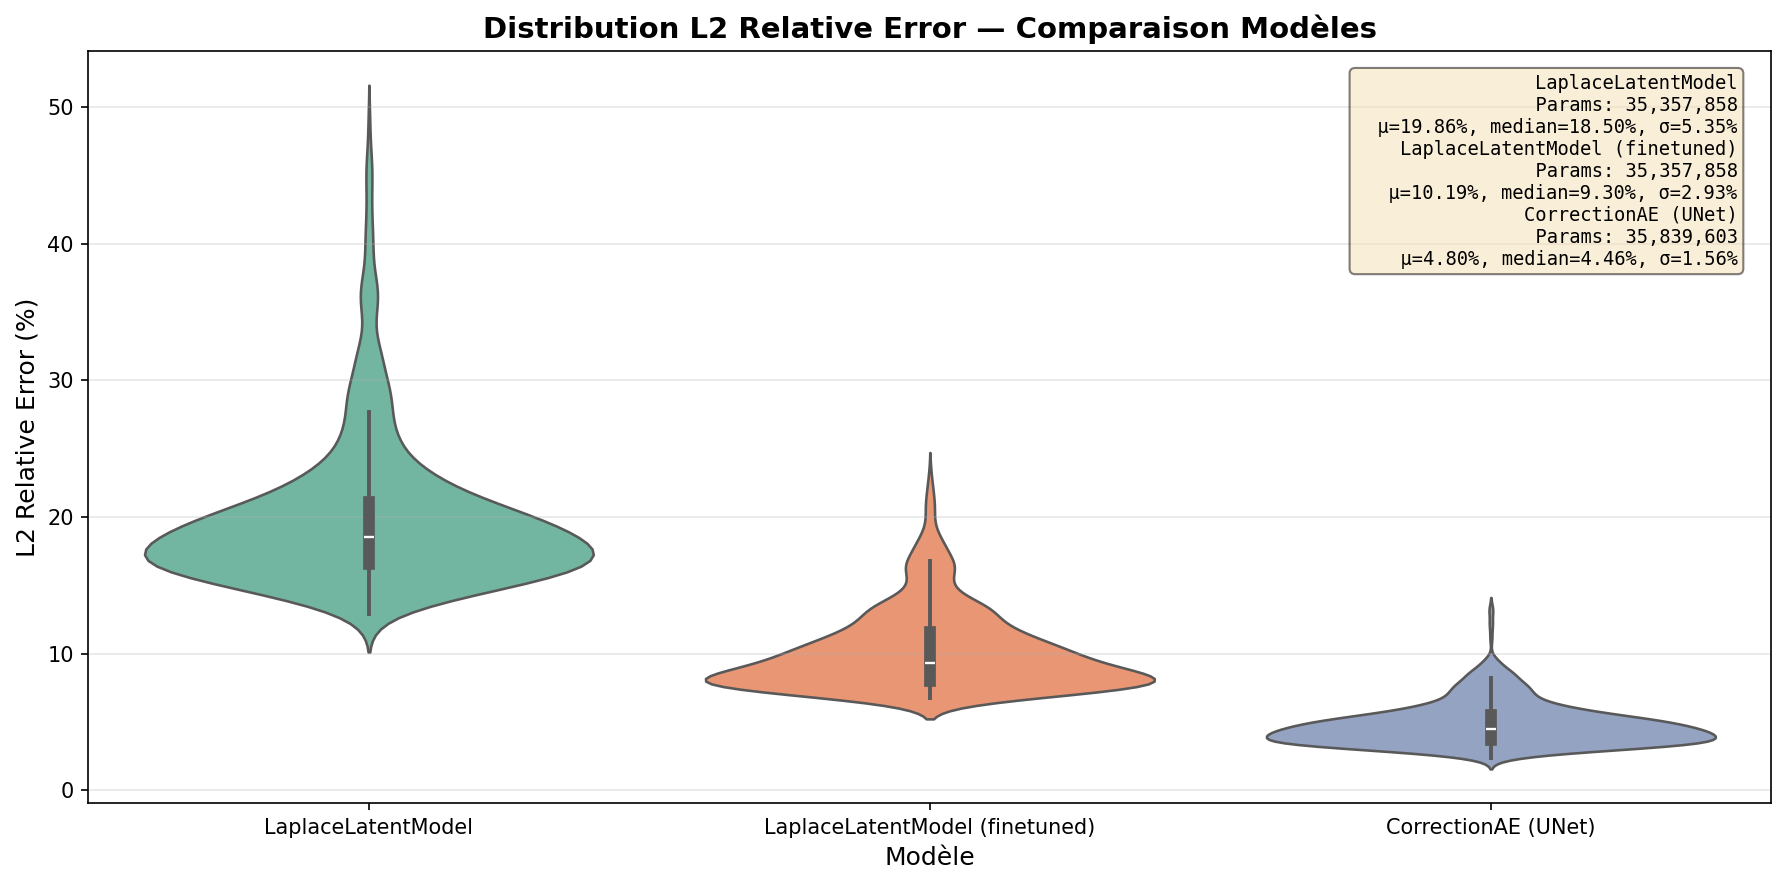
\includegraphics[height=4.8cm]{benchmark_l2rel.png}
      \caption{Benchmark performance comparison}
  \end{figure}
\end{frame}

\begin{frame}{Conclusion}
  \textbf{Key Takeaways:}
  \begin{itemize}
      \item \textbf{Laplace Domain Decomposition:} Solves the memory bottleneck effectively, matching non-linear dynamics without losing spatial resolution.
      \item \textbf{Frequency-Conditioned Model:} Effectively builds a continuous non-linear space shared among complex frequencies.
      \item \textbf{End-to-End Fine-Tuning:} Absolutely indispensable for circumventing decoding bottlenecks (-50\% error).
      \item \textbf{Post-Hoc Residual Correction:} A lightweight solution for eliminating spectral truncation footprints (-52\% further error reduction).
  \end{itemize}
\end{frame}

\section{Ongoing \& Future Work}

\begin{frame}{Regularised Inversion \& Bias-Variance Trade-off}
  \textbf{1. Regularised Inverse Problem}\\
  Penalize amplitudes and spatio-temporal gradients via $\mathbf{L}_{\mathrm{reg}}$:
  \vspace{-0.5em}
  \begin{align*}
      \hat{\mathbf{v}}^* &= \arg\min_{\mathbf{v}} \|\mathbf{F}_{st}\mathbf{v} - \hat{\mathbf{u}}\|^2 + \mathbf{v}^\top \mathbf{L}_{\mathrm{reg}} \mathbf{v} \\
      \underbrace{(\mathbf{F}_{st}^H\mathbf{F}_{st} + \mathbf{L}_{\mathrm{reg}})}_{=:\,\mathbf{A}} \hat{\mathbf{v}}^* &= \mathbf{F}_{st}^H \hat{\mathbf{u}}
  \end{align*}
  
  \textbf{2. Exact Error Decomposition}\\
  Let $\mathbf{u} = \mathbf{F}_{st}\mathbf{v}$ and $\mathbf{v}^* = \mathbf{A}^{-1}\mathbf{F}_{st}^H\mathbf{u}$. The total error splits analytically:
  \vspace{-0.5em}
  \[ \mathbf{v} - \hat{\mathbf{v}}^* = \underbrace{\mathbf{A}^{-1}\mathbf{L}_{\mathrm{reg}}\mathbf{v}}_{\text{Regularisation Bias}} \;+\; \underbrace{\mathbf{A}^{-1}\mathbf{F}_{st}^H (\mathbf{u} - \hat{\mathbf{u}})}_{\text{Propagated Variance}} \]
  
  \textbf{3. Bias-Variance Bound}\\
  \vspace{-0.5em}
  \[ \|\mathbf{v} - \hat{\mathbf{v}}^*\| \leq \|\mathbf{v} - \mathbf{v}^*\| + \underbrace{\|\mathbf{A}^{-1}\mathbf{F}_{st}^H\|}_{\text{Condition number}} \cdot \underbrace{\|\mathbf{u} - \hat{\mathbf{u}}\|}_{\text{Surrogate error}} \]
\end{frame}

\begin{frame}{SVD Residual as a Proxy Objective}
  \small
  \begin{itemize}
      \item Direct AE error evaluation is computationally intractable.
      \item \textbf{Method:} We define a grid in the complex Laplace domain ($s_k \in \mathbb{C}$). For each grid point, we train a small AE (1,000 samples) \& compute linear SVD residual.
  \end{itemize}
  \vspace{-0.5em}
  \begin{columns}[T]
      \column{0.32\textwidth}
      \begin{figure}
          \centering
          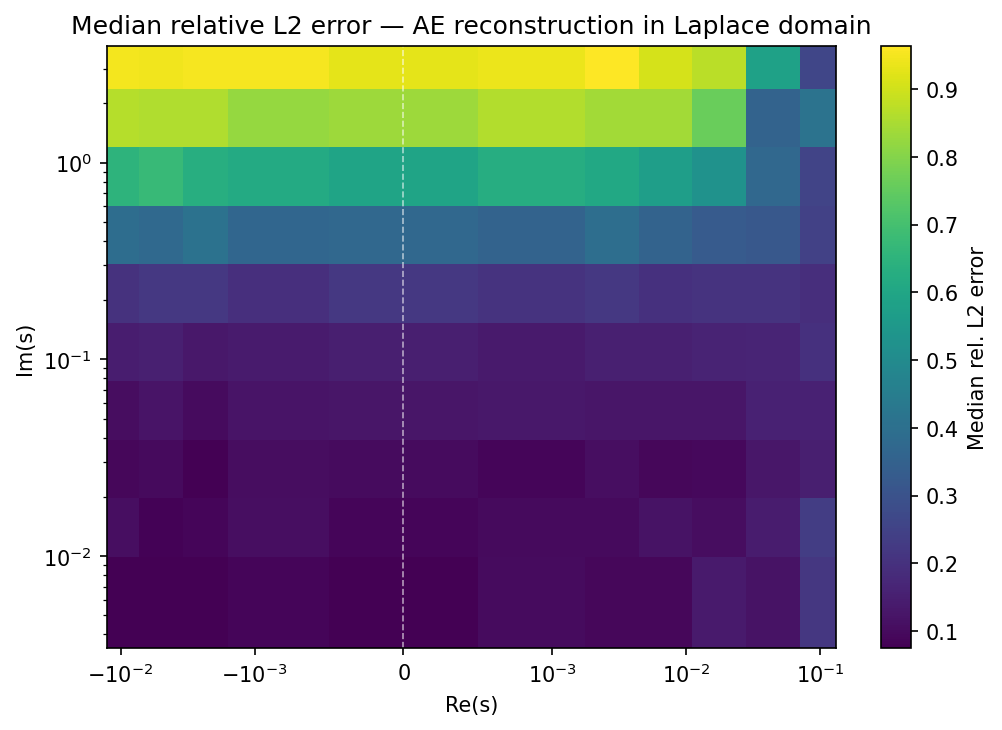
\includegraphics[width=\linewidth, height=3.5cm, keepaspectratio]{error_map.png}
          \caption{AE Val Error Map}
      \end{figure}
      \column{0.32\textwidth}
      \begin{figure}
          \centering
          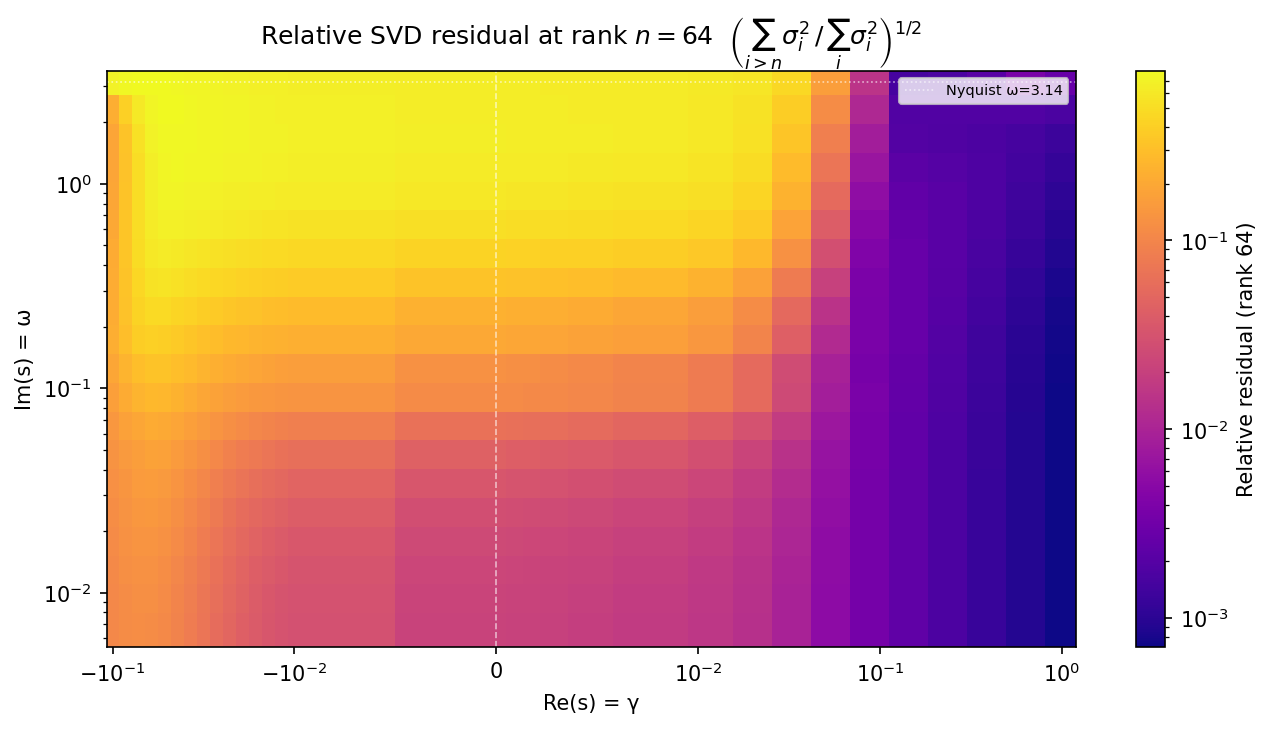
\includegraphics[width=\linewidth, height=3.5cm, keepaspectratio]{laplace_svd_residual.png}
          \caption{SVD Residual Grid}
      \end{figure}
      \column{0.32\textwidth}
      \begin{figure}
          \centering
          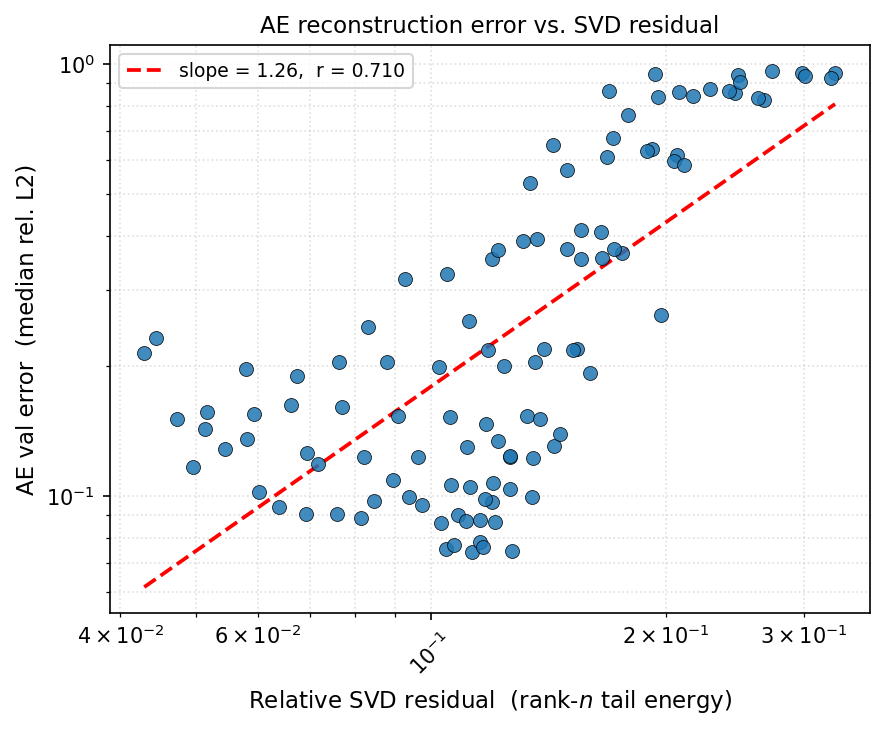
\includegraphics[width=\linewidth, height=3.5cm, keepaspectratio]{laplace_error_svd_correlation.png}
          \caption{Correlation}
      \end{figure}
  \end{columns}
  \vspace{-0.5em}
  \textbf{Conclusion:} Strong correlation validates the SVD residual as a differentiable proxy objective.
\end{frame}

\begin{frame}{Contour Optimization via SVD Proxy Objective}
  \textbf{1. Surrogate Error Approximation}\\
  Evaluating $\|\mathbf{u}-\hat{\mathbf{u}}\|$ requires training an AE for each contour $\mathbf{s}$. We approximate it via the mean SVD residual (optimal linear surrogate of rank $r$):
  \vspace{-0.5em}
  \[ \epsilon_{\mathrm{AE}}(\mathbf{s}) \;\approx\; \mathcal{E}_{\mathrm{SVD}}(\mathbf{s}) \;=\; \sqrt{ \frac{1}{|\Theta|} \sum_{s_i \in \mathbf{s}} \sum_{j > r} \bigl(\sigma_j^{(s_i)}\bigr)^2 } \]
  
  \textbf{2. Final Differentiable Proxy Objective}\\
  Jointly optimize $\mathbf{s}$ and regularisation parameters $(\lambda, \alpha)$ using the scaled proxy:
  \vspace{-0.5em}
  \begin{align*}
      \mathcal{L}^{\mathrm{proxy}}(\mathbf{s}, \lambda, \alpha) \;&=\; \underbrace{\frac{1}{|\Theta|} \sum_{\theta \in \Theta} \|\mathbf{v}(\theta) - \mathbf{v}^*(\theta)\|}_{\text{Expected Bias}}
      \quad + \underbrace{\frac{1}{\lambda_{\mathrm{AE}}} \|\mathbf{A}^{-1}\mathbf{F}_{st}^H\| \cdot \mathcal{E}_{\mathrm{SVD}}(\mathbf{s})}_{\text{Expected Variance Proxy}} \\
      &\quad + \underbrace{\lambda_x \|\nabla (\mathbf{v}^* -\mathbf{v})\| + \lambda_t \|\partial_t (\mathbf{v}^* -\mathbf{v})\|}_{\text{Artifact heuristics}}
  \end{align*}
\end{frame}

\begin{frame}{Differentiable Contour Optimization}
  \begin{columns}[c]
      \column{0.35\textwidth}
      \textbf{Optimization framework:}
      \begin{itemize}
          \item \textbf{PyTorch} proxy $\mathcal{L}^{\mathrm{proxy}}$
          \item \textbf{Auto-diff} w.r.t $\mathbf{s \in \mathbb{C}}$
          \item \textbf{AdamW} optimizer
          \item With $L_{reg}$ = $\lambda I$ + $\alpha_t D_t$, the problem is separable in x : we optimize pixel par pixel (memory efficient)
      \end{itemize}
      \column{0.65\textwidth}
      \centering
      \begin{minipage}{0.48\textwidth}
          \begin{figure}
              \centering
              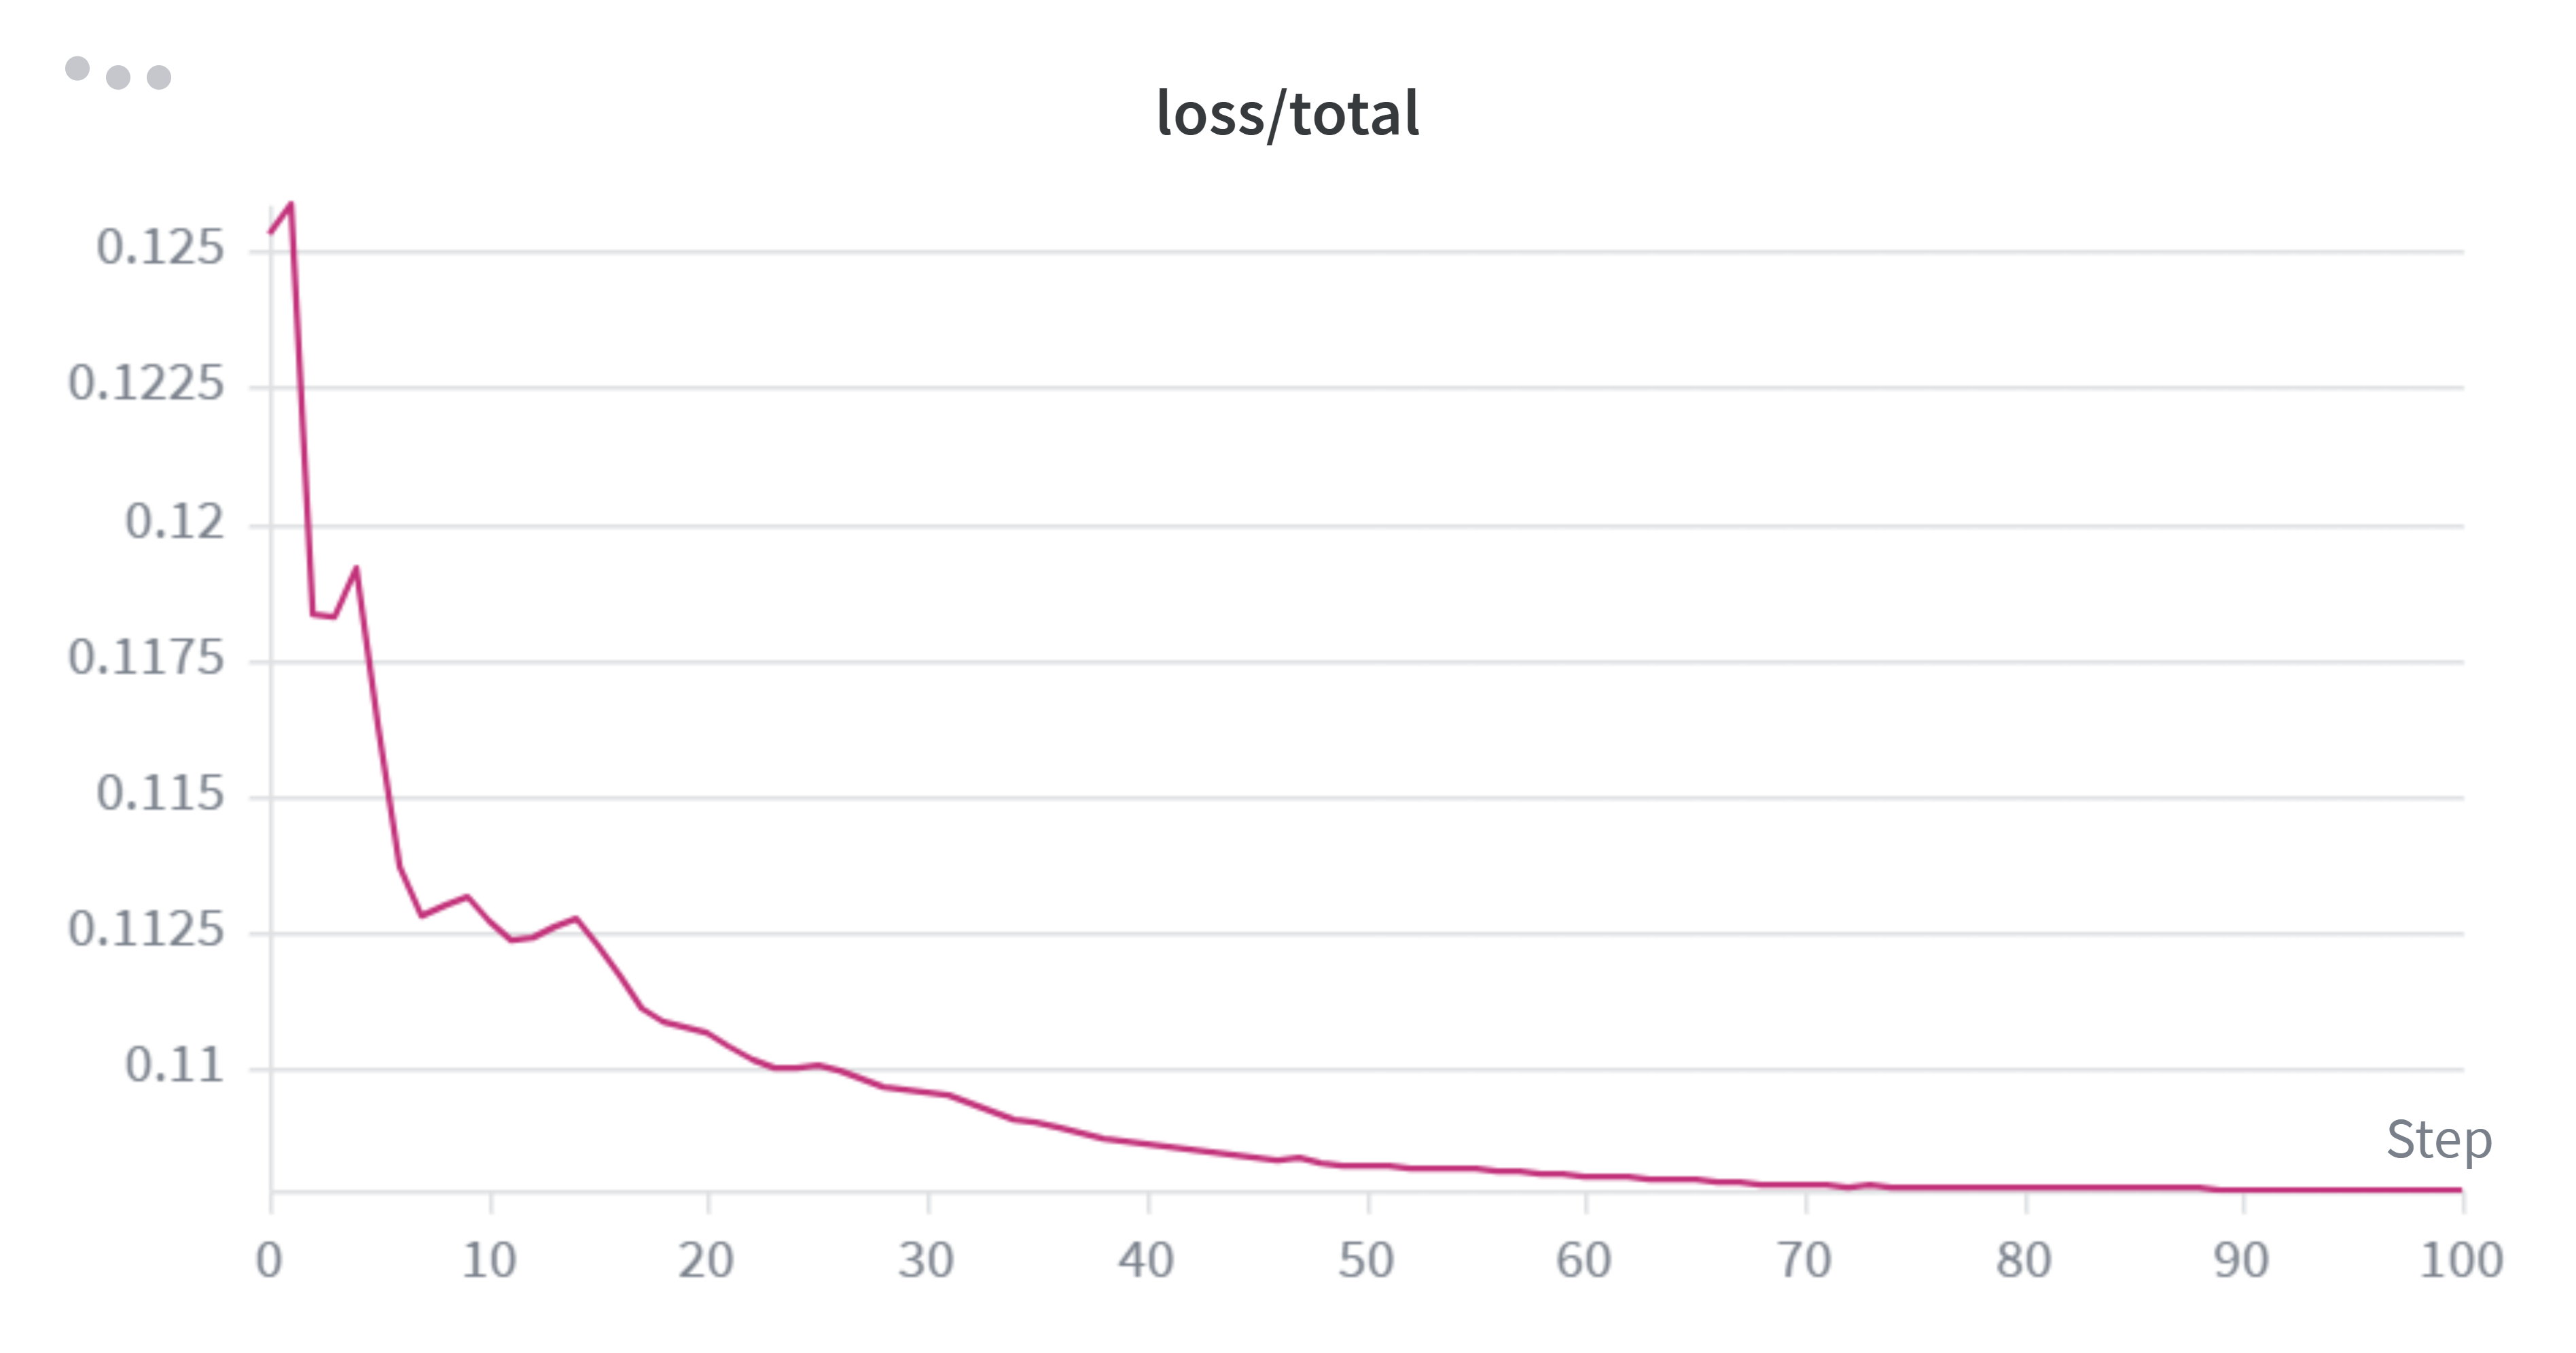
\includegraphics[width=\linewidth, height=2.8cm, keepaspectratio]{loss_s_opti.png}
              \caption{Total Proxy Loss}
          \end{figure}
      \end{minipage}
      \hfill
      \begin{minipage}{0.48\textwidth}
          \begin{figure}
              \centering
              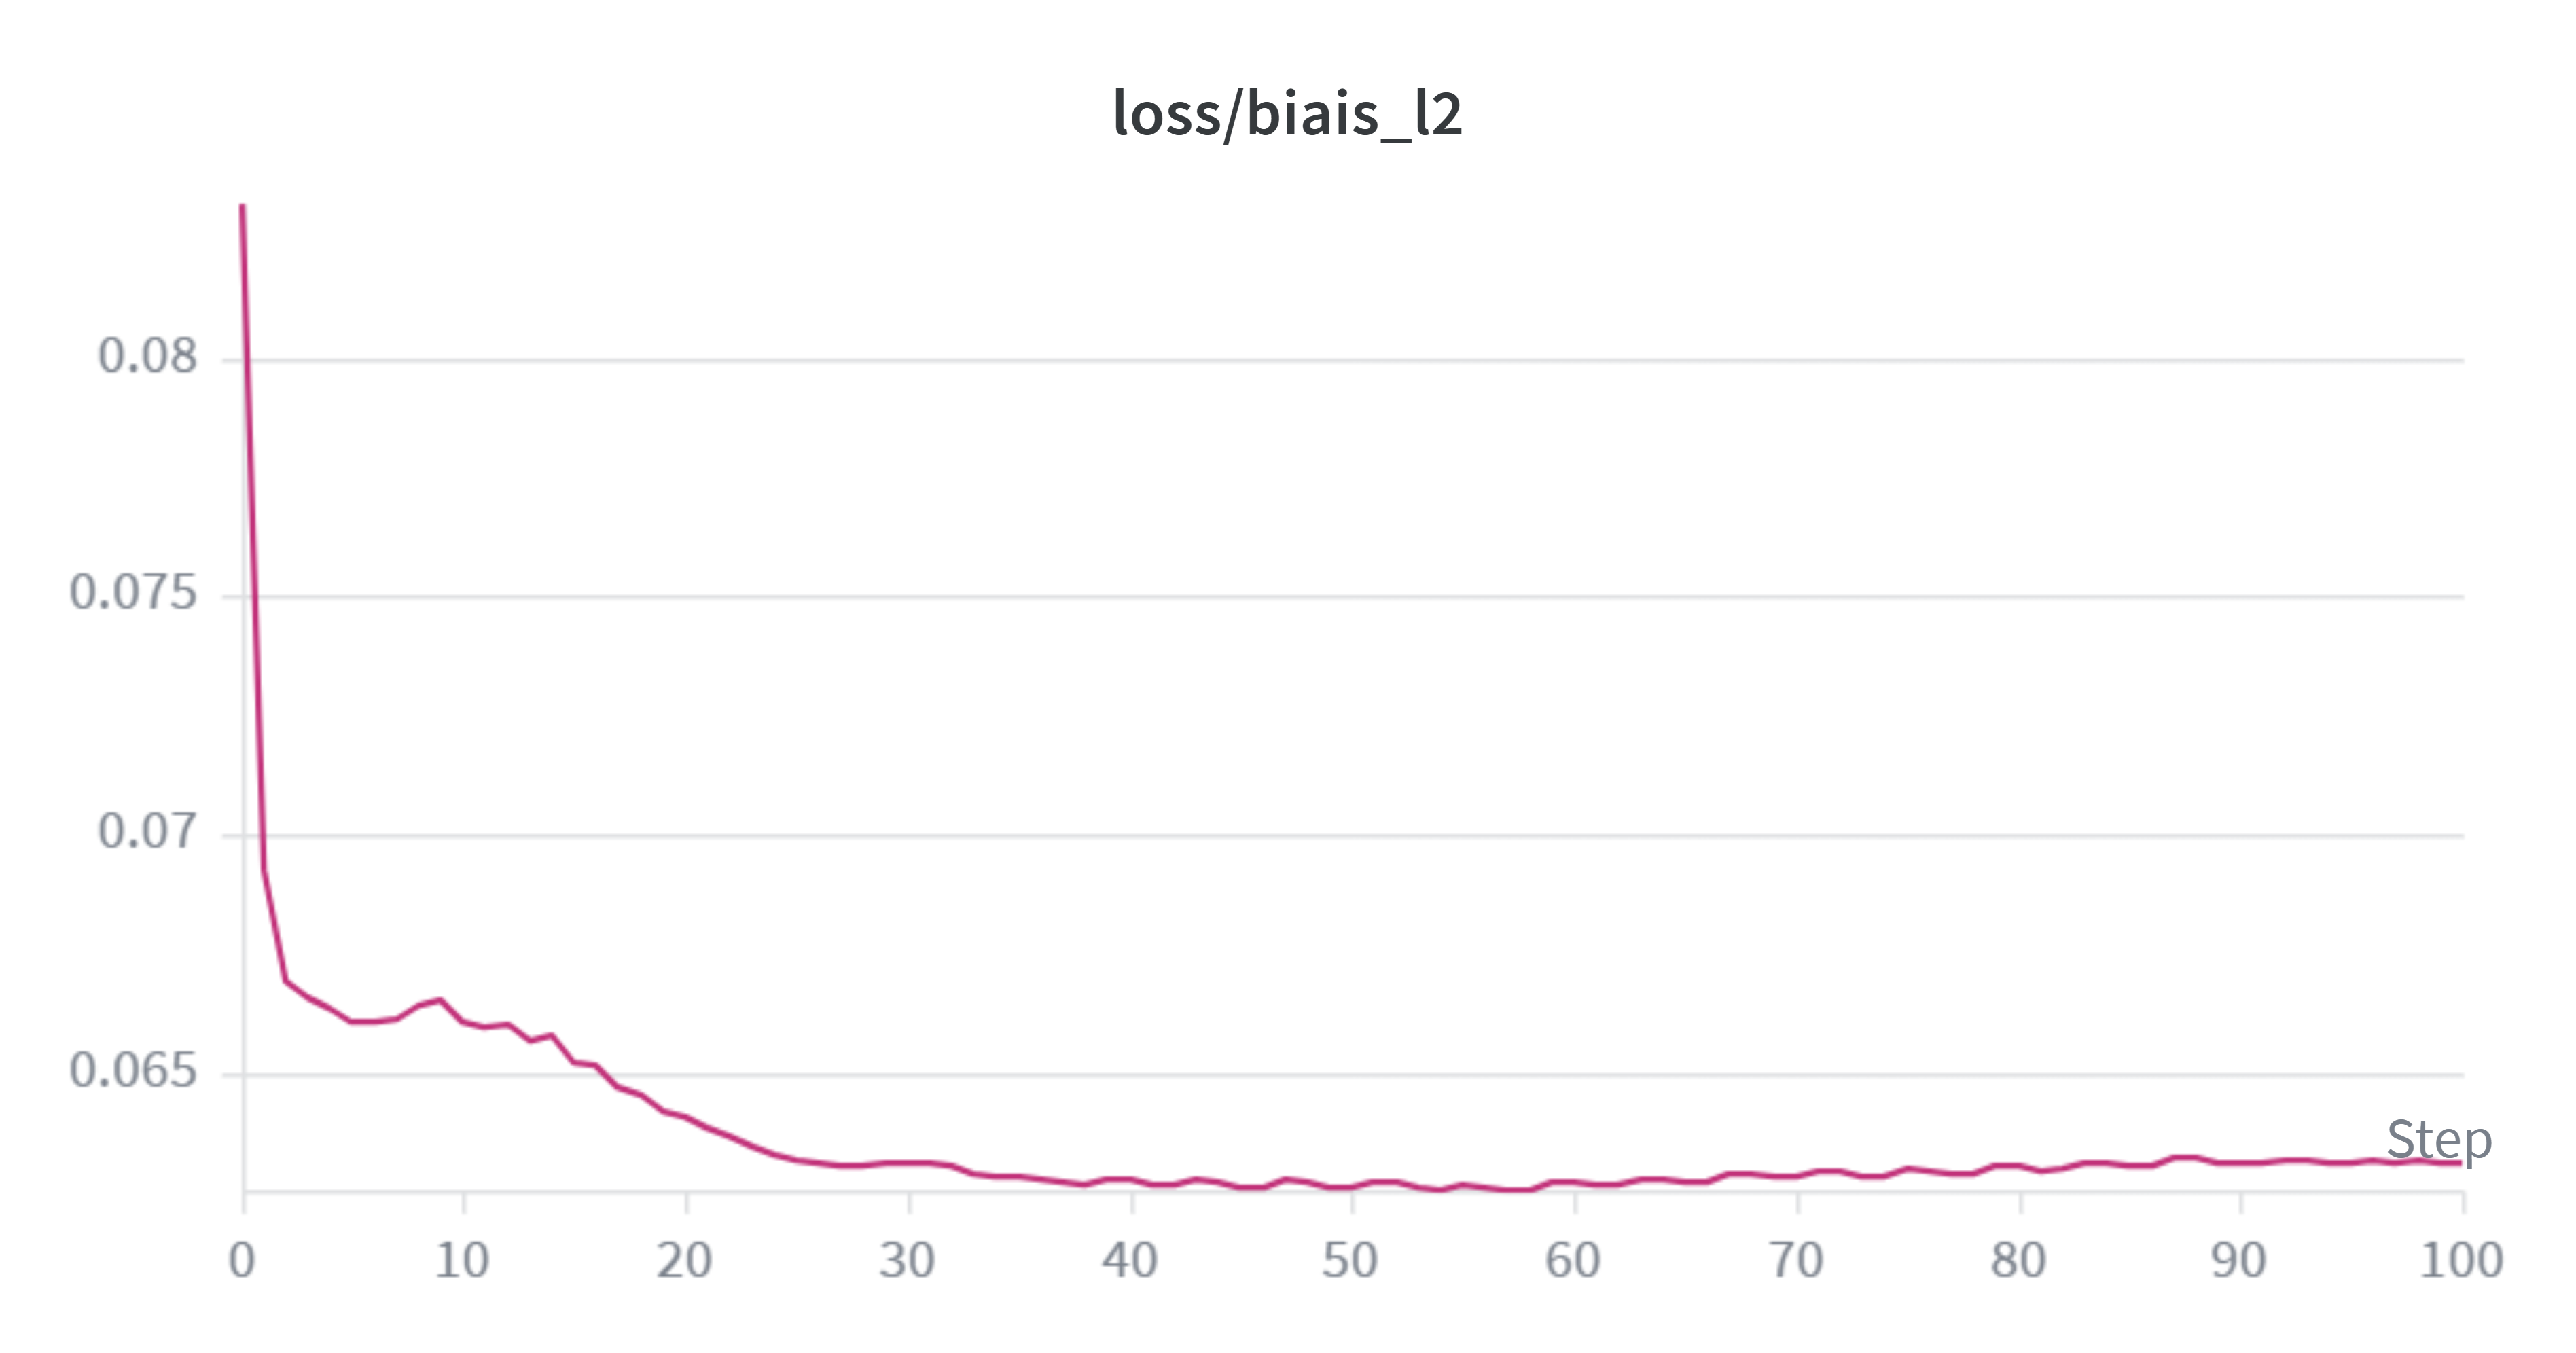
\includegraphics[width=\linewidth, height=2.8cm, keepaspectratio]{l2_s_opti.png}
              \caption{Regularisation Bias}
          \end{figure}
      \end{minipage}
      
      \vspace{0.4em}
      
      \begin{minipage}{0.48\textwidth}
          \begin{figure}
              \centering
              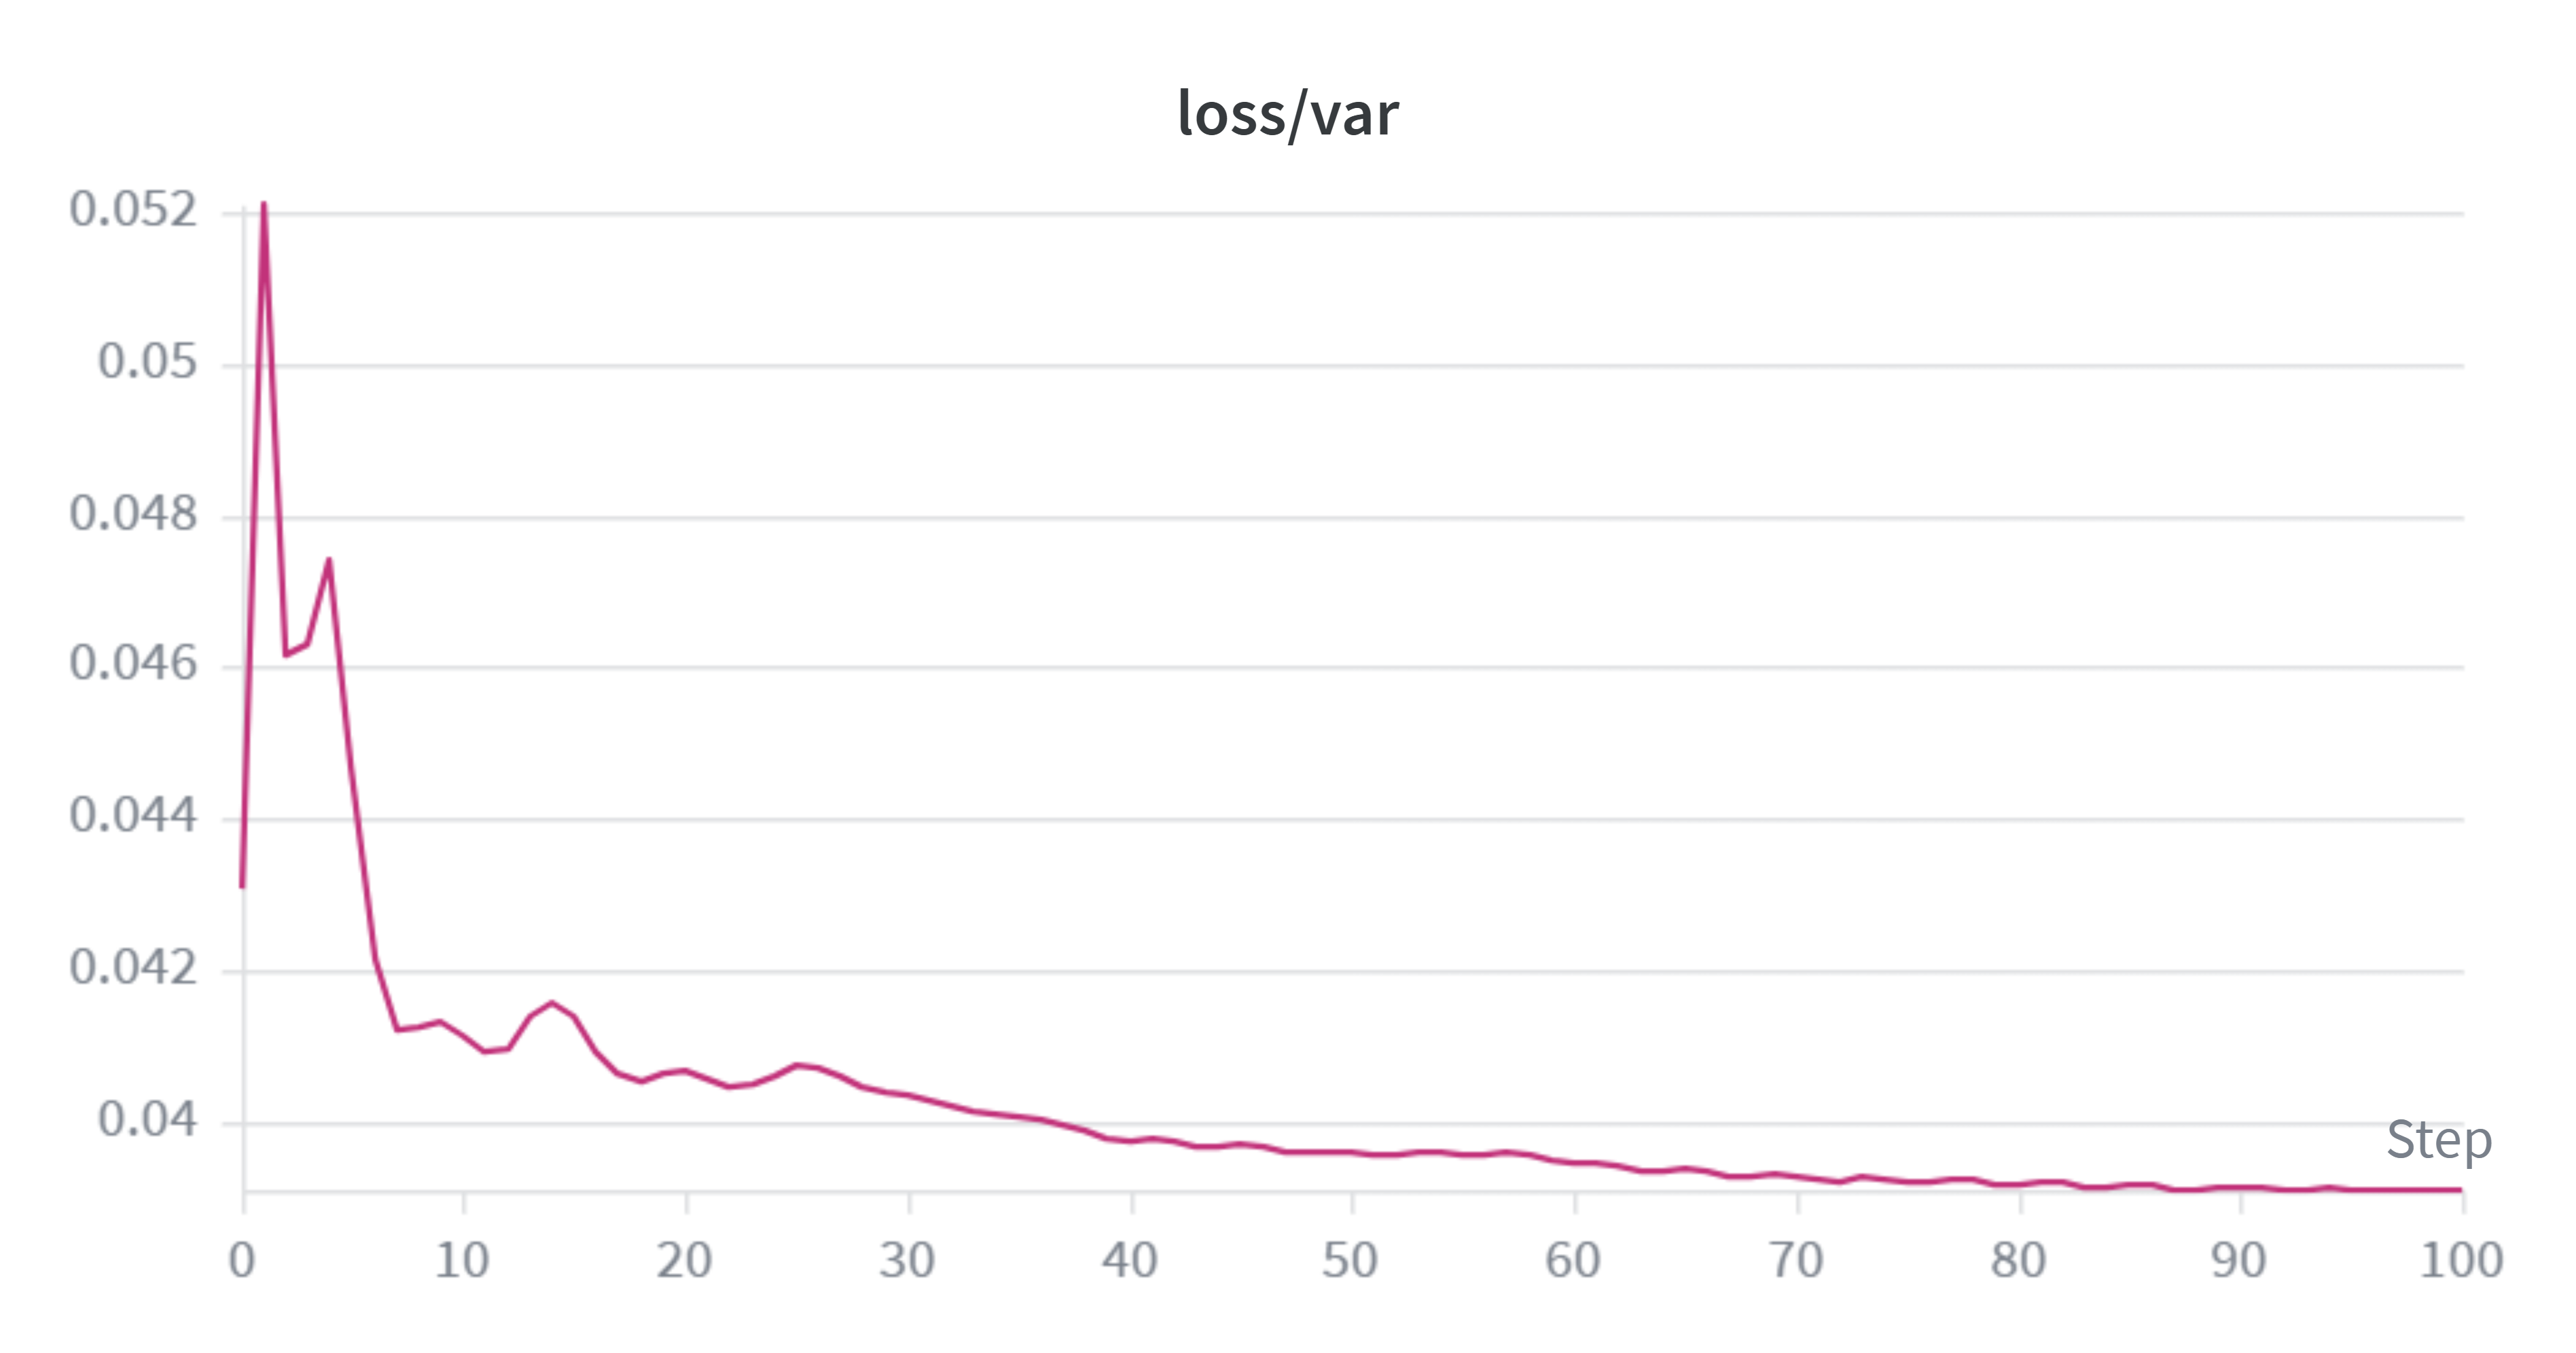
\includegraphics[width=\linewidth, height=2.8cm, keepaspectratio]{var_s_opti.png}
              \caption{SVD Variance Proxy}
          \end{figure}
      \end{minipage}
      \hfill
      \begin{minipage}{0.48\textwidth}
          \begin{figure}
              \centering
              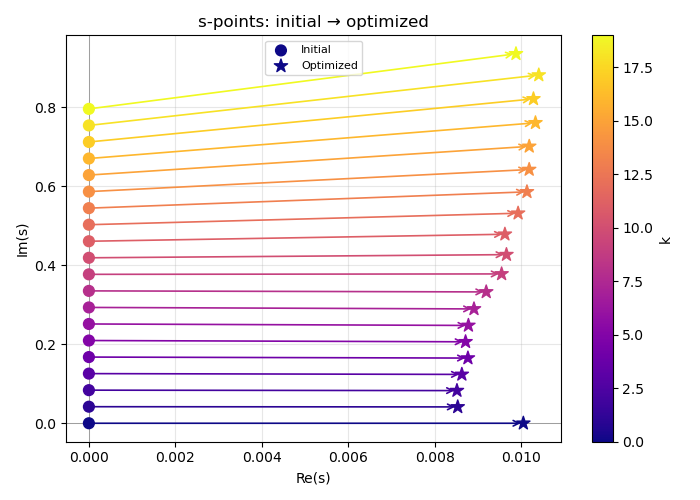
\includegraphics[width=\linewidth, height=2.8cm, keepaspectratio]{s_opti.png}
              \caption{Contour Trajectory}
          \end{figure}
      \end{minipage}
  \end{columns}
\end{frame}

\begin{frame}{Impact on Laplace SVD Model}
  \begin{columns}
      \column{0.5\textwidth}
      \begin{figure}
          \centering
          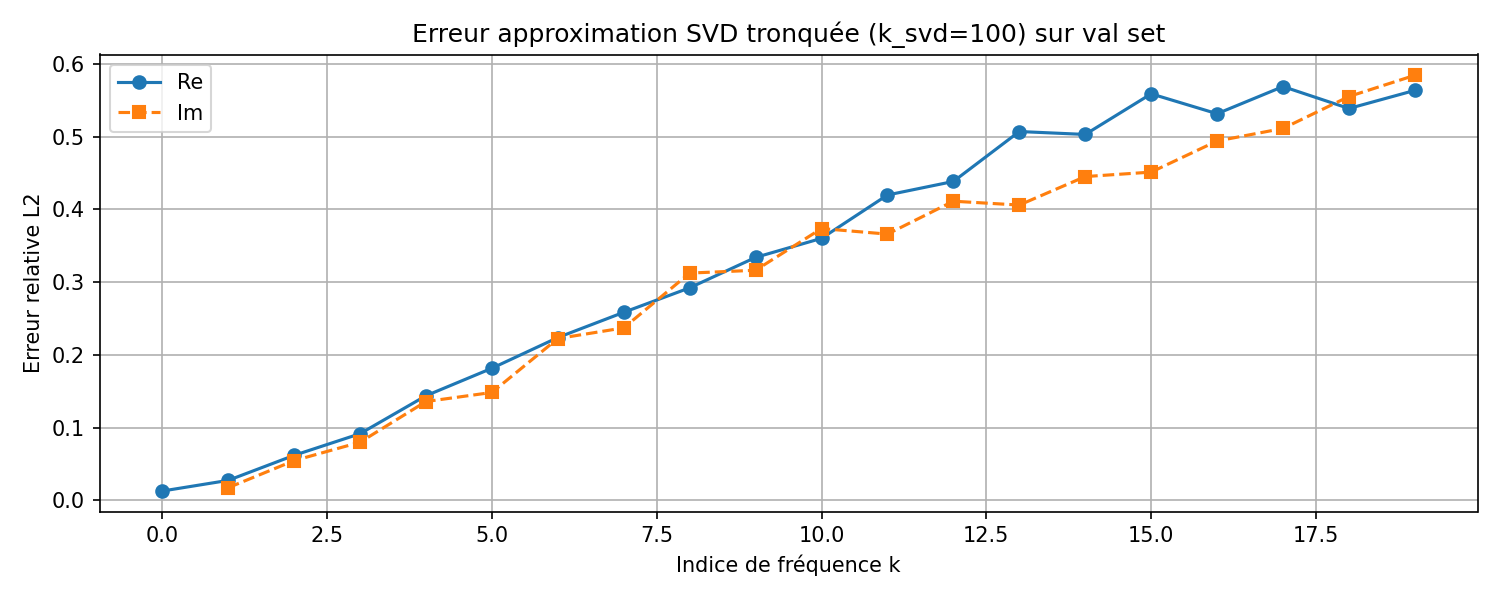
\includegraphics[width=\linewidth, keepaspectratio]{LaplaceSVDModel_svd_error_ksvd100.png}
          \caption{Standard SVD error}
      \end{figure}
      \column{0.5\textwidth}
      \begin{figure}
          \centering
          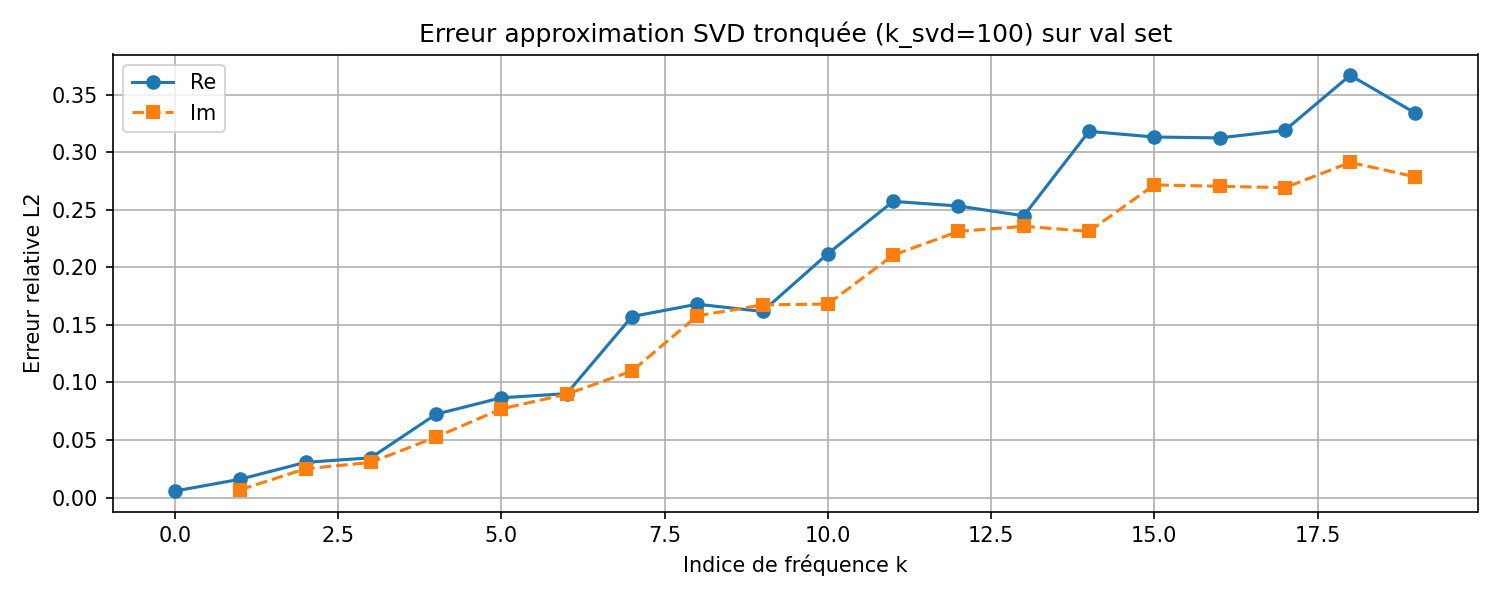
\includegraphics[width=\linewidth, keepaspectratio]{LaplaceSVDModel_svd_error_ksvd100_optimal.png}
          \caption{Optimized SVD error}
      \end{figure}
  \end{columns}
  Consequent improvement : using SVD on Laplace maps is now possible. 
  
  \textbf{Limitation} : $\theta \to c(\theta)$ is hard to learn.
\end{frame}

\begin{frame}{Impact on Laplace AE Model}
  \vspace{-0.5em}
  \begin{columns}[T]
      \column{0.5\textwidth}
      \centering
      \textbf{Loss Comparison}
      \begin{figure}
          \centering
          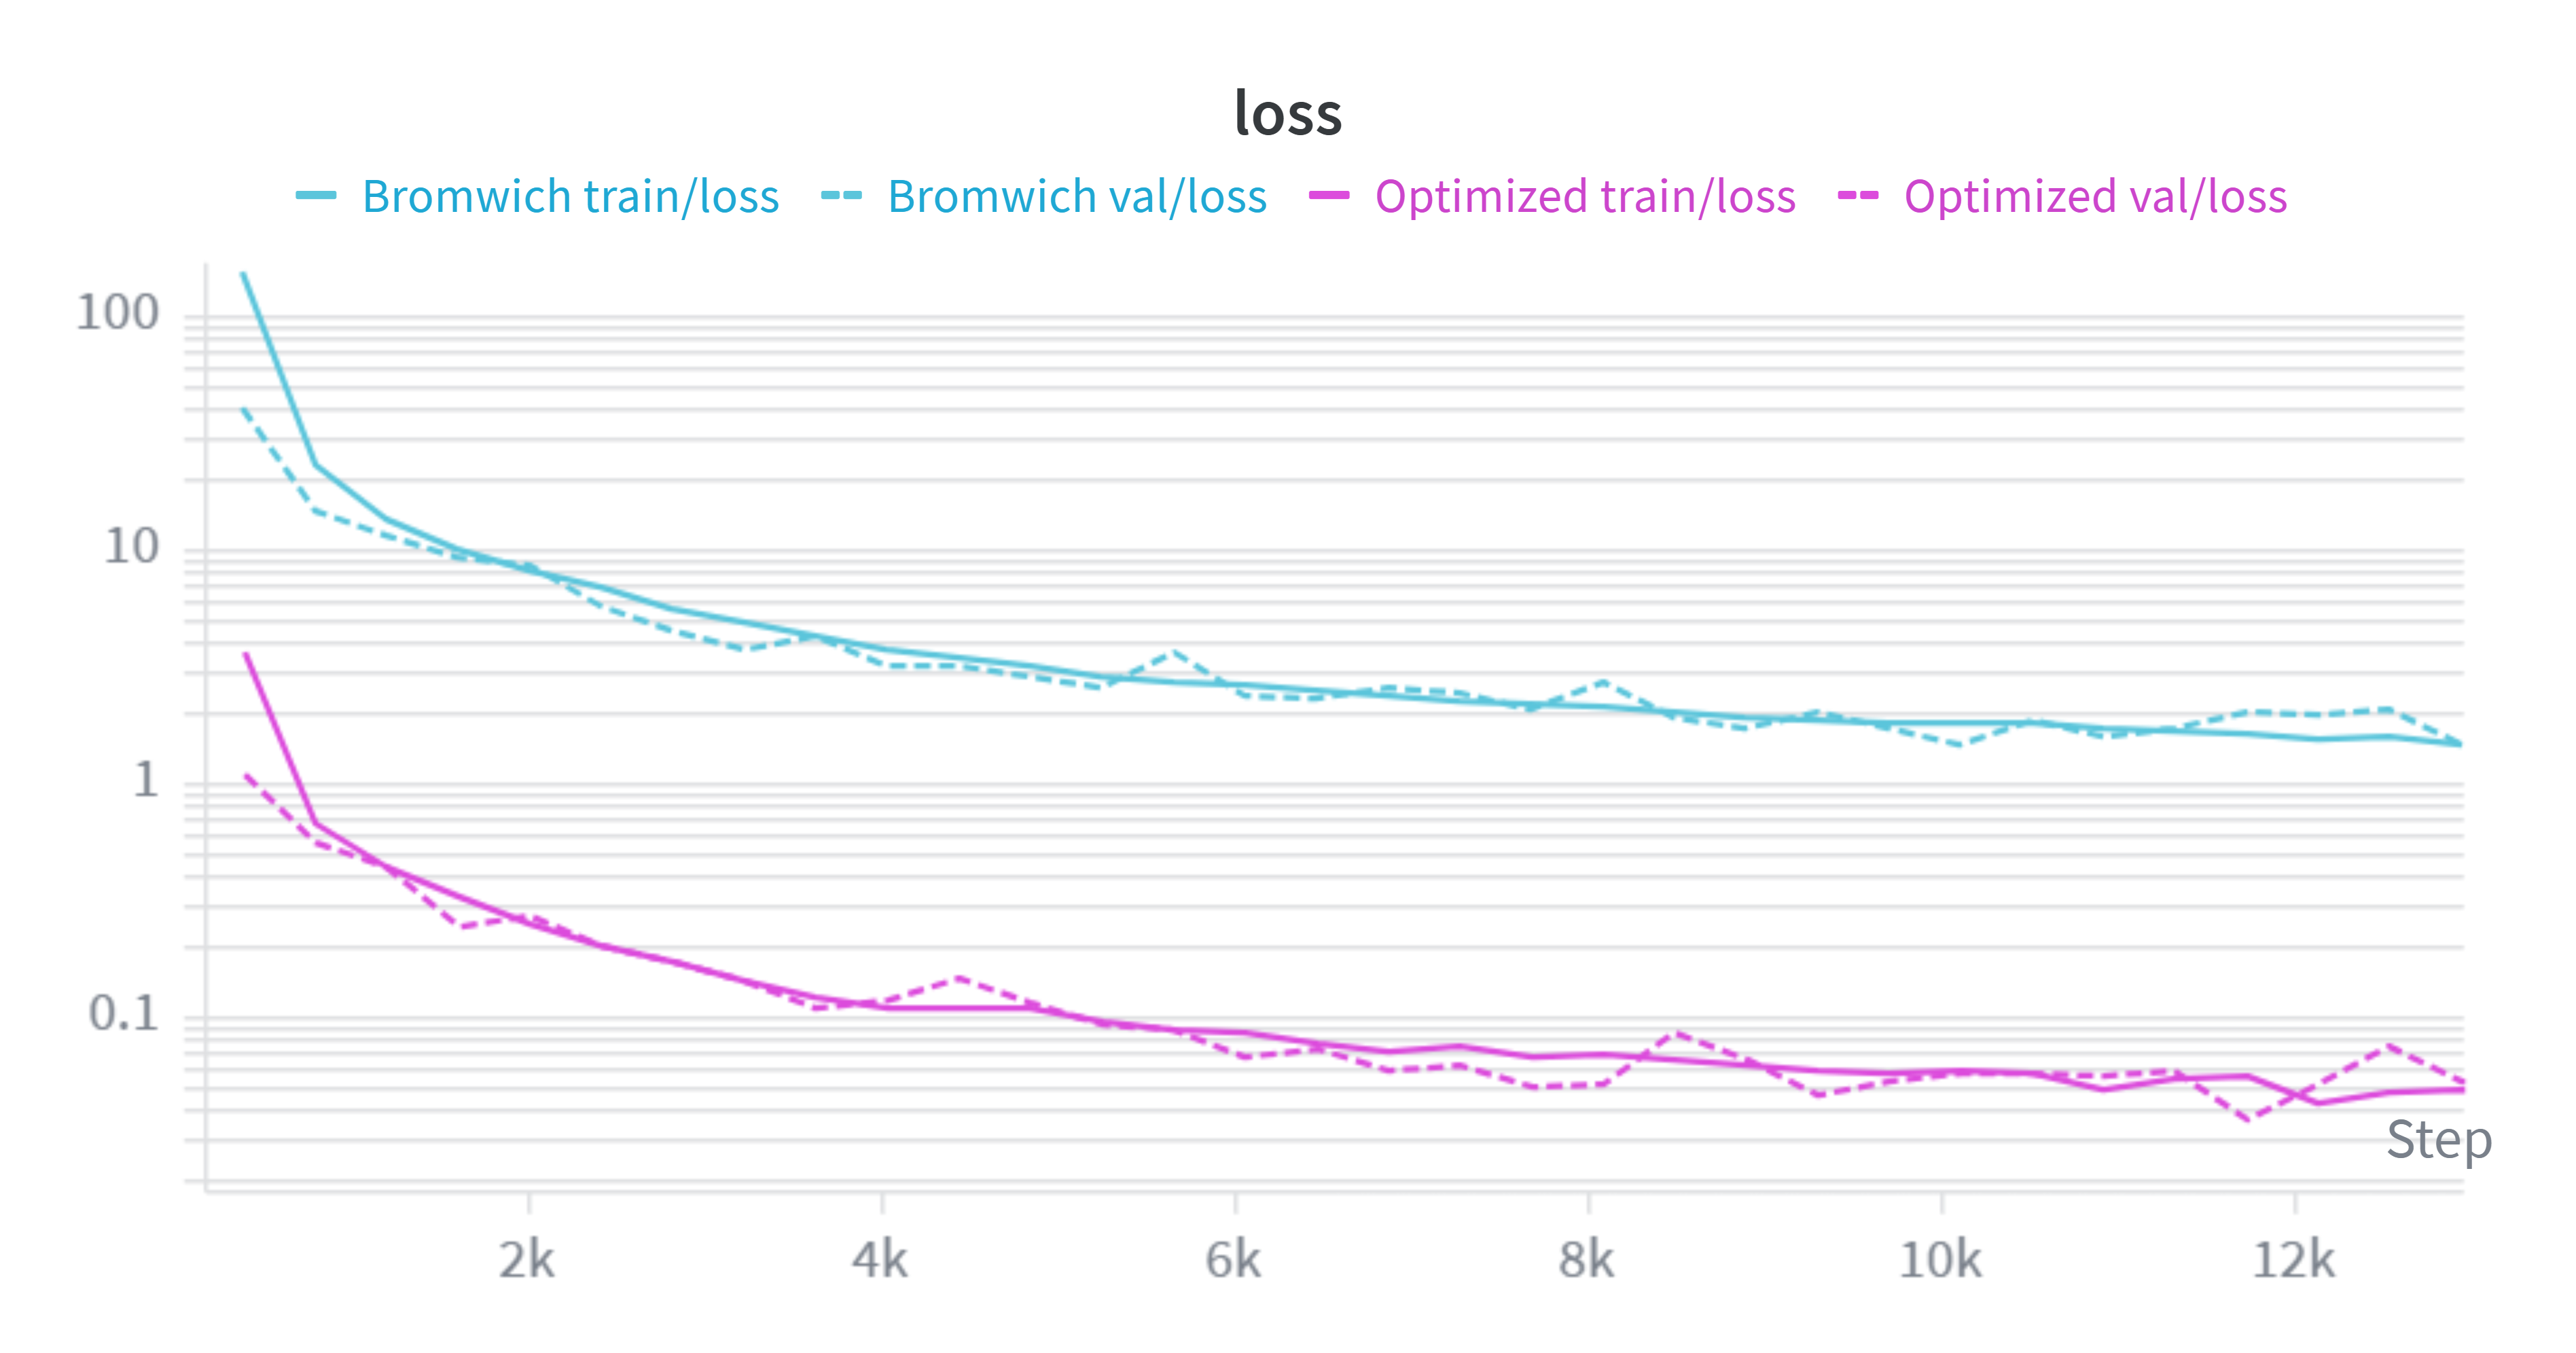
\includegraphics[width=\linewidth, height=5cm, keepaspectratio]{loss comparison.png}
          \caption{Proxy Loss vs AE Loss}
      \end{figure}
      
      \column{0.48\textwidth}
      \centering
      \textbf{Temporal Error}
      \vspace{-0.5em}
      \begin{figure}
          \centering
          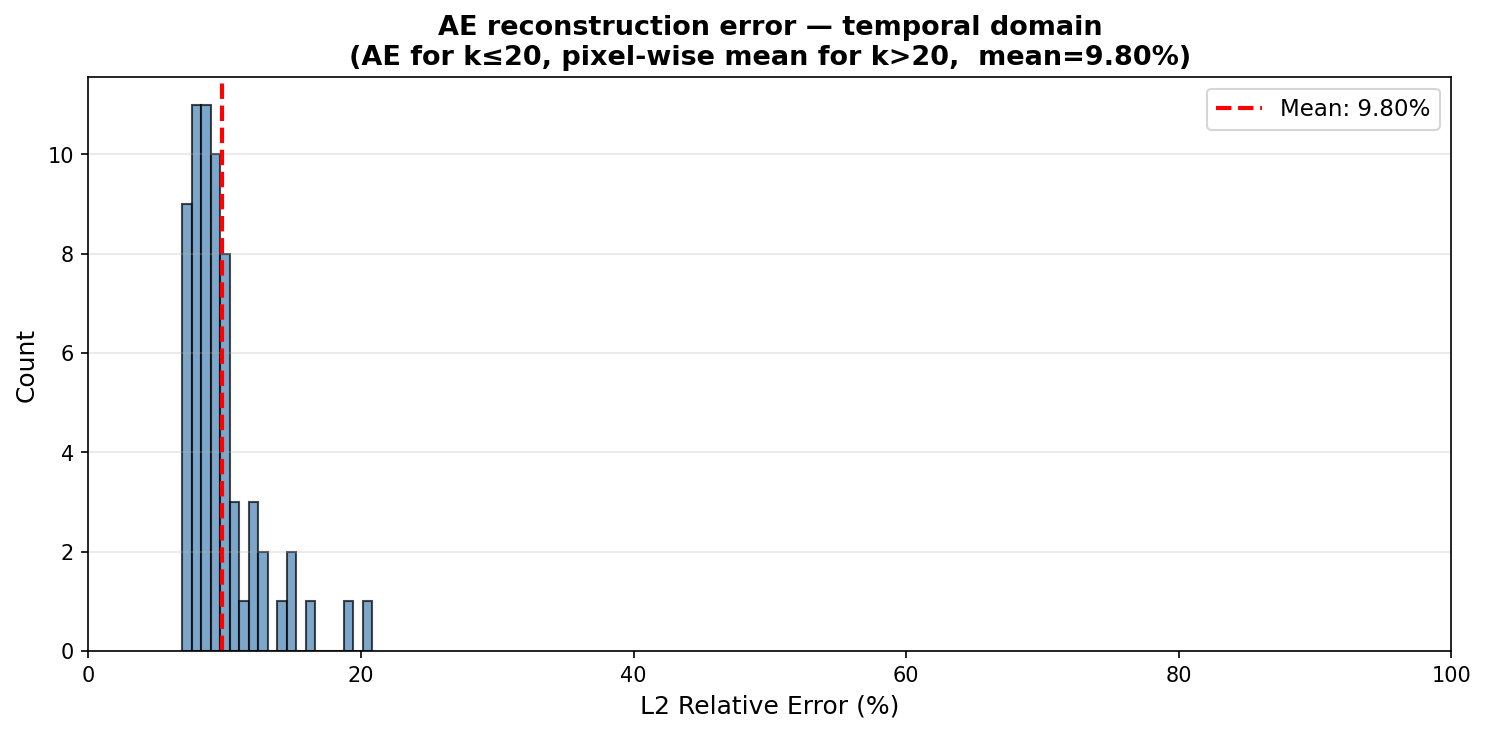
\includegraphics[width=\linewidth, height=2.3cm, keepaspectratio]{ae_study_temporal_error.png}
          \caption{Standard Contour}
      \end{figure}
      \vspace{-1.5em}
      \begin{figure}
          \centering
          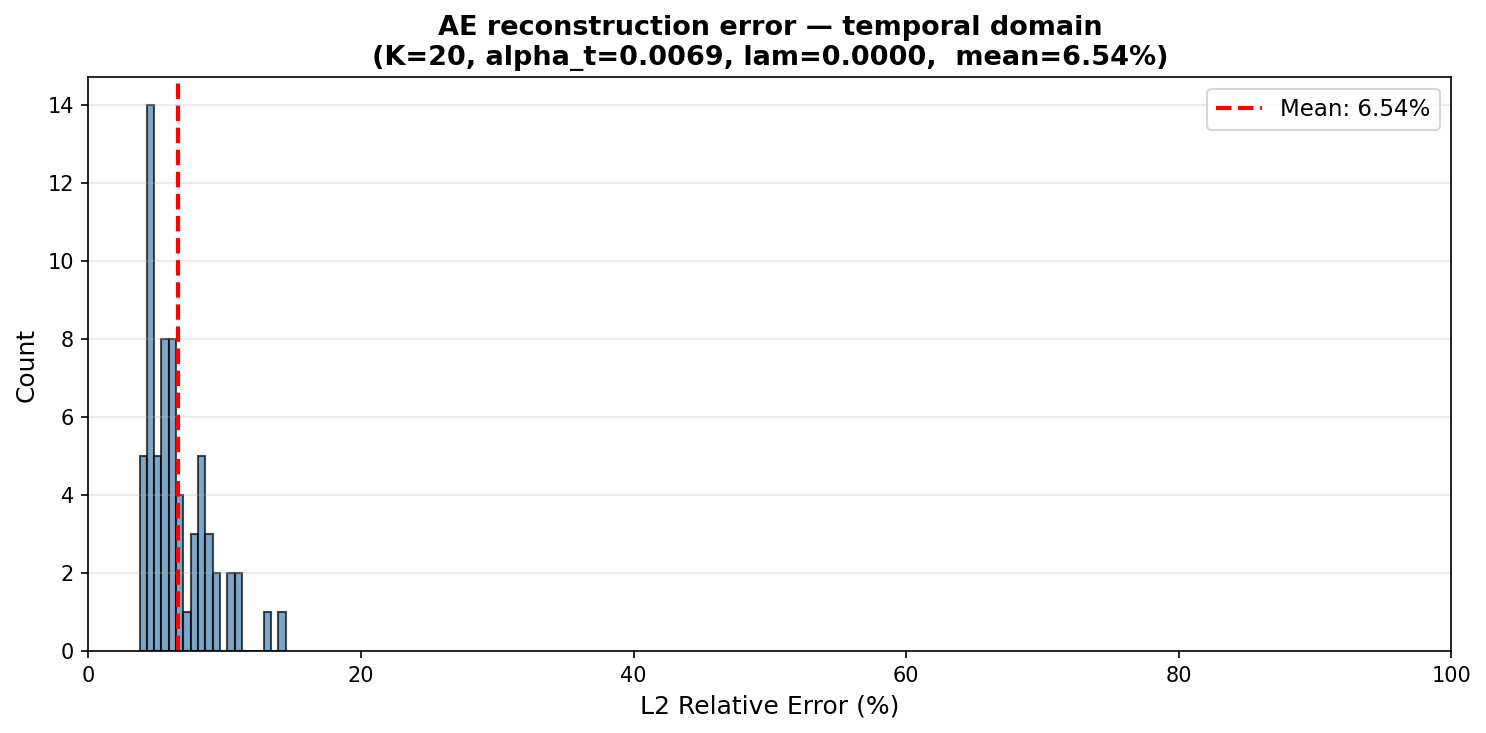
\includegraphics[width=\linewidth, height=2.3cm, keepaspectratio]{opti_ae_study_temporal_error.png}
          \caption{Optimized Contour}
      \end{figure}
  \end{columns}
  \vspace{-0.2em}
  \textbf{Conclusion:} Mean error drops from 9.94\% to 6.50\% ($\sim$30\% improvement).
\end{frame}

\begin{frame}{Limitations \& Perspectives (1/2): Frequency Error}
  \begin{itemize}
      \item \textbf{Frequency Error:} Opti better for $k < 5$, but worse at high frequencies.
      \item \textbf{Truncation ($k_{\max}=20$):} High tail error despite low energy $\implies$ likely too large.
  \end{itemize}
  
  \vspace{0.5em}
  \begin{columns}[T]
      \column{0.48\textwidth}
      \begin{figure}
          \centering
          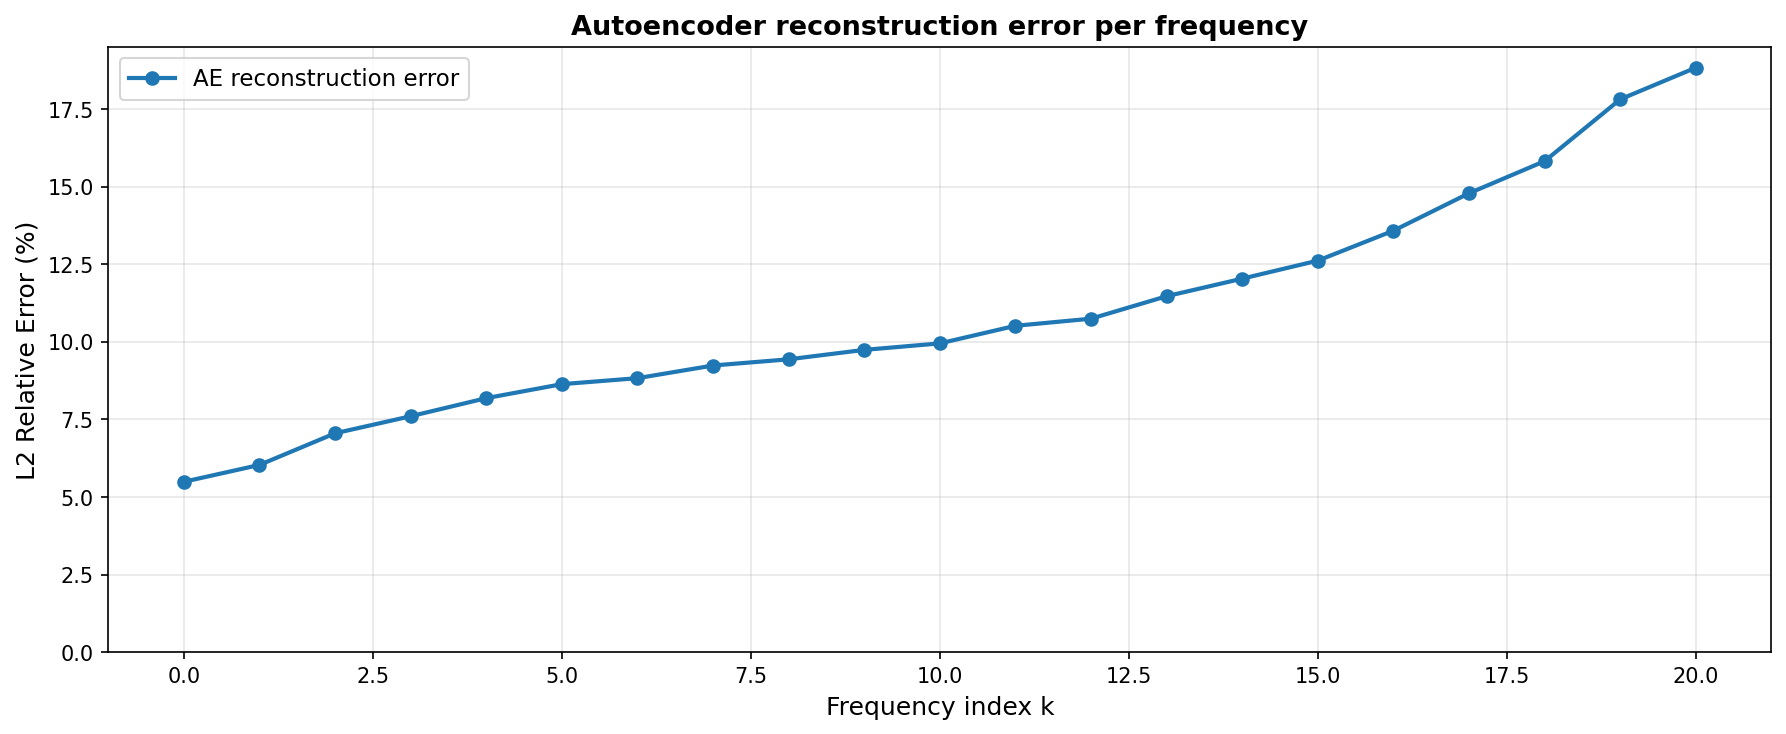
\includegraphics[width=\linewidth, height=3.8cm, keepaspectratio]{ae_study_frequency_error.png}
          \caption{Freq Error (Std)}
      \end{figure}
      \column{0.48\textwidth}
      \begin{figure}
          \centering
          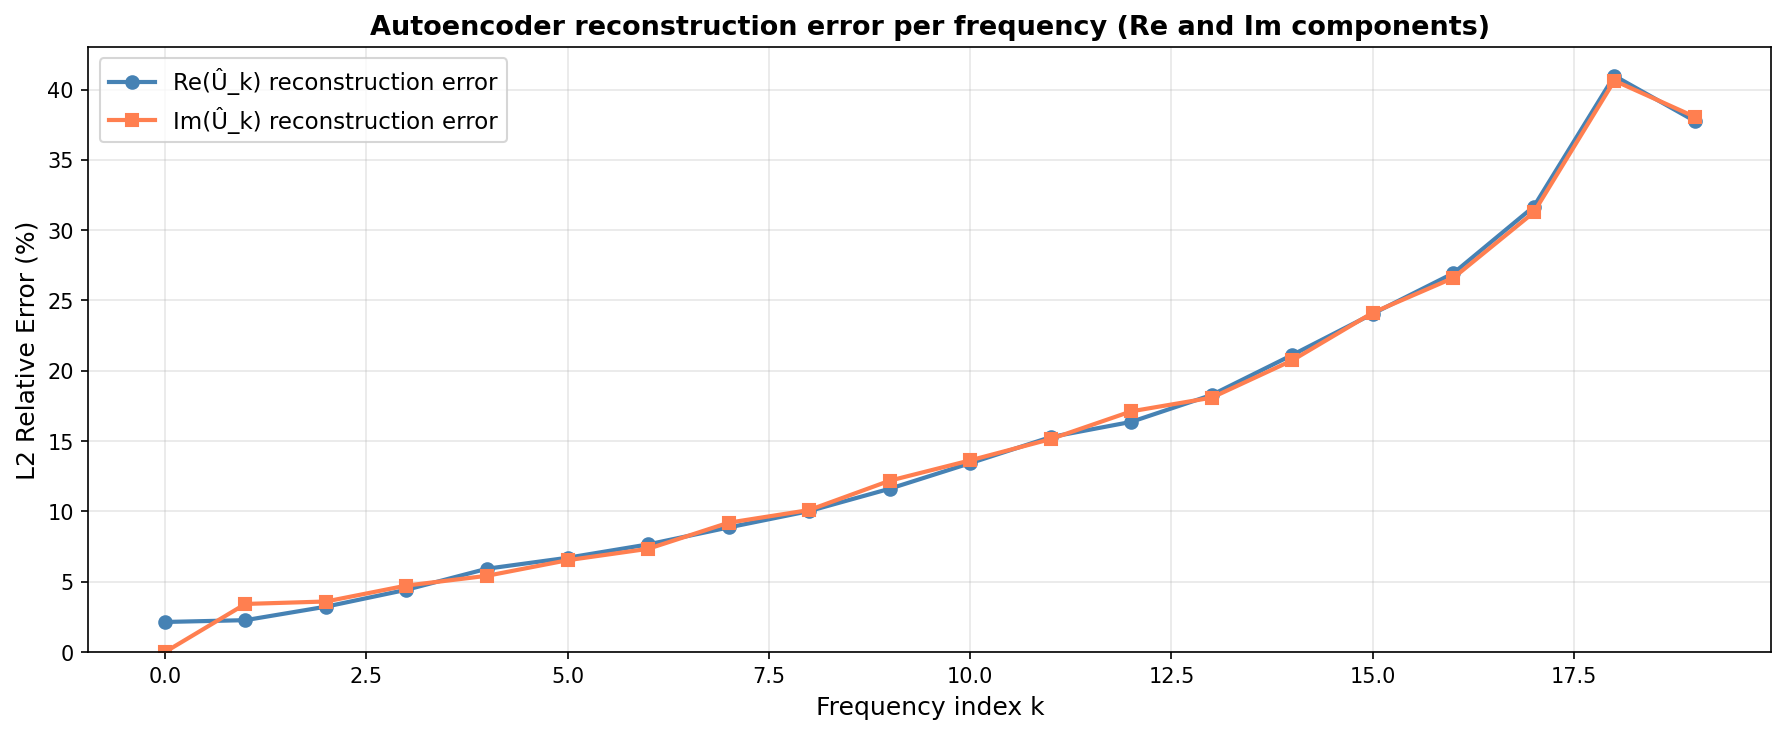
\includegraphics[width=\linewidth, height=3.8cm, keepaspectratio]{opti_ae_study_frequency_error.png}
          \caption{Freq Error (Opti)}
      \end{figure}
  \end{columns}
\end{frame}

\begin{frame}{Limitations \& Perspectives (2/2): Pure Reconstruction}
  \begin{itemize}
      \item \textbf{Pure Reconstruction:} Standard FFT ($\gamma = 0$) outperforms optimized Laplace contour.
      \item \textbf{Next Step:} Should we apply FFT parameterized along a specific optimized path?
  \end{itemize}
  
  \vspace{0.5em}
  \begin{columns}[T]
      \column{0.48\textwidth}
      \begin{figure}
          \centering
          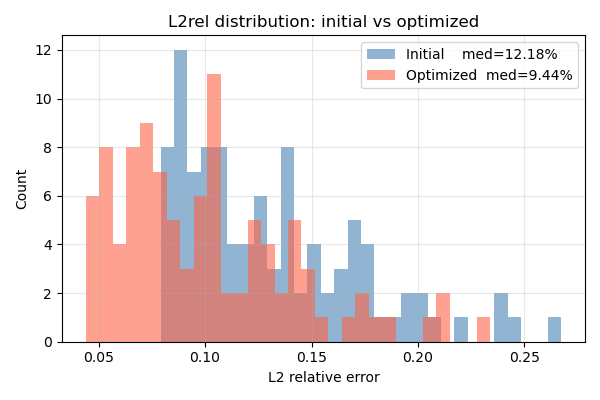
\includegraphics[width=\linewidth, height=3.8cm, keepaspectratio]{l2hist_s_opti.png}
          \caption{Reconstruction (Opti)}
      \end{figure}
      \column{0.48\textwidth}
      \begin{figure}
          \centering
          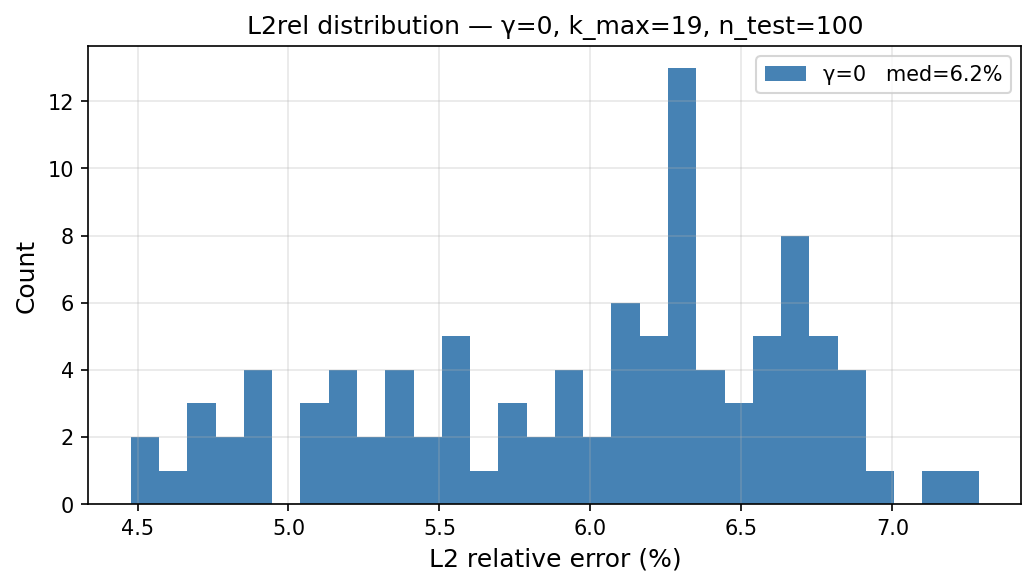
\includegraphics[width=\linewidth, height=3.8cm, keepaspectratio]{gamma_opti_hist.png}
          \caption{Reconstruction (FFT)}
      \end{figure}
  \end{columns}
\end{frame}
\begin{frame}{State of the Art \& Next Work}
  \begin{itemize}
      \item \textbf{Laplace Operators (Field-to-Field)}
      \begin{itemize}
          \item Unresolved challenge: explicit time management.
          \item Laplace transform is an interesting approach to this issue (already used, but mainly as an operator).
      \end{itemize}
      \vspace{0.5em}
      \item \textbf{Model Order Reduction}
      \begin{itemize}
          \item \textit{Current work:} Classic use of Proper Orthogonal Decomposition (POD) and Autoencoders (AE).
          \item Laplace reduction is rarer. Time management faces the same issues as above, often handled by treating time simply as an additional variable.
      \end{itemize}
  \end{itemize}
\end{frame}

\begin{frame}{Related Work: MOR via Contour Integrals}
  \textbf{Ref:} \textit{Model Order Reduction in Contour Integral Methods for Parametric PDEs}
  
  \vspace{1em}
  \begin{itemize}
      \item \textbf{Method:} Projection-based MOR using Laplace transform for parametric linear PDEs.
      \item \textbf{Direct Time Evaluation:} Contour quadrature evaluates solutions at specific instants.
      \item \textbf{POD Efficiency:} Drastically reduces snapshot count by skipping intermediate time steps.
      \item \textbf{Main Achievement:} Circumvents slow singular value decay (Kolmogorov $N$-width) for linear advection equations.
  \end{itemize}
\end{frame}


\begin{frame}
  \begin{center}
      \Huge \textbf{Thank you!}
  \end{center}
\end{frame}

\end{document}
